% !TeX root = main.tex

% main.tex
% header.tex
\documentclass[a4paper,11pt,twoside,ngerman,xcolor]{book}
\usepackage[a4paper,left=3.5cm,right=2.5cm,bottom=3.5cm,top=3cm]{geometry}

\usepackage[german,english]{babel}

\usepackage[pdftex]{graphicx,xcolor}
\usepackage{amsmath,amssymb,subfigure}

\usepackage{pdfpages}
\usepackage[hidelinks]{hyperref}


% Theorem-Umgebungen
\usepackage[amsmath,thmmarks]{ntheorem}

% Korrekte Darstellung der Umlaute
\usepackage[utf8]{inputenc}
\usepackage[T1]{fontenc}

% Algorithmen
\usepackage[chapter]{algorithm}
\usepackage{algorithmic}

\usepackage{enumerate}


% Bibtex deutsch
\usepackage{bibgerm}
\usepackage[numbers]{natbib}

% URLs
\usepackage{url}

% Caption Packet
\usepackage[margin=0pt,font=small,labelfont=bf]{caption}
% Gliederung einstellen
%\setcounter{secnumdepth}{5}
%\setcounter{tocdepth}{5}

% Theorem-Optionen %
\theoremseparator{.}
\theoremstyle{change}
\newtheorem{theorem}{Theorem}[section]
\newtheorem{satz}[theorem]{Satz}
\newtheorem{lemma}[theorem]{Lemma}
\newtheorem{korollar}[theorem]{Korollar}
\newtheorem{proposition}[theorem]{Proposition}
% Ohne Numerierung
\theoremstyle{nonumberplain}
\renewtheorem{theorem*}{Theorem}
\renewtheorem{satz*}{Satz}
\renewtheorem{lemma*}{Lemma}
\renewtheorem{korollar*}{Korollar}
\renewtheorem{proposition*}{Proposition}
% Definitionen mit \upshape
\theorembodyfont{\upshape}
\theoremstyle{change}
\newtheorem{definition}[theorem]{Definition}
\theoremstyle{nonumberplain}
\renewtheorem{definition*}{Definition}
% Kursive Schrift
\theoremheaderfont{\itshape}
\newtheorem{notation}{Notation}
\newtheorem{konvention}{Konvention}
\newtheorem{bezeichnung}{Bezeichnung}
\theoremsymbol{\ensuremath{\Box}}
\newtheorem{beweis}{Beweis}
\theoremsymbol{}
\theoremstyle{change}
\theoremheaderfont{\bfseries}
\newtheorem{bemerkung}[theorem]{Bemerkung}
\newtheorem{beobachtung}[theorem]{Beobachtung}
\newtheorem{beispiel}[theorem]{Beispiel}
\newtheorem{problem}{Problem}
\theoremstyle{nonumberplain}
\renewtheorem{bemerkung*}{Bemerkung}
\renewtheorem{beispiel*}{Beispiel}
\renewtheorem{problem*}{Problem}

% Algorithmen anpassen %
\renewcommand{\algorithmicrequire}{\textit{Eingabe:}}
\renewcommand{\algorithmicensure}{\textit{Ausgabe:}}
\floatname{algorithm}{Algorithmus}
\renewcommand{\listalgorithmname}{Algorithmenverzeichnis}
\renewcommand{\algorithmiccomment}[1]{\textcolor{gray}{// #1}}

% Zeilenabstand einstellen %
\renewcommand{\baselinestretch}{1.25}
% Floating-Umgebungen anpassen %
\renewcommand{\topfraction}{0.9}
\renewcommand{\bottomfraction}{0.8}
% Abkuerzungen richtig formatieren %
\usepackage{xspace}
\newcommand{\vgl}{vgl.\@\xspace} 
\newcommand{\zB}{z.\nolinebreak[4]\hspace{0.125em}\nolinebreak[4]B.\@\xspace}
\newcommand{\bzw}{bzw.\@\xspace}
\newcommand{\dahe}{d.\nolinebreak[4]\hspace{0.125em}h.\nolinebreak[4]\@\xspace}
\newcommand{\etc}{etc.\@\xspace}
\newcommand{\evtl}{evtl.\@\xspace}
\newcommand{\ggf}{ggf.\@\xspace}
\newcommand{\bzgl}{bzgl.\@\xspace}
\newcommand{\so}{s.\nolinebreak[4]\hspace{0.125em}\nolinebreak[4]o.\@\xspace}
\newcommand{\iA}{i.\nolinebreak[4]\hspace{0.125em}\nolinebreak[4]A.\@\xspace}
\newcommand{\sa}{s.\nolinebreak[4]\hspace{0.125em}\nolinebreak[4]a.\@\xspace}
\newcommand{\su}{s.\nolinebreak[4]\hspace{0.125em}\nolinebreak[4]u.\@\xspace}
\newcommand{\ua}{u.\nolinebreak[4]\hspace{0.125em}\nolinebreak[4]a.\@\xspace}
\newcommand{\og}{o.\nolinebreak[4]\hspace{0.125em}\nolinebreak[4]g.\@\xspace}
\newcommand{\oBdA}{o.\nolinebreak[4]\hspace{0.125em}\nolinebreak[4]B.\nolinebreak[4]\hspace{0.125em}d.\nolinebreak[4]\hspace{0.125em}A.\@\xspace}
\newcommand{\OBdA}{O.\nolinebreak[4]\hspace{0.125em}\nolinebreak[4]B.\nolinebreak[4]\hspace{0.125em}d.\nolinebreak[4]\hspace{0.125em}A.\@\xspace}

% Leere Seite ohne Seitennummer, naechste Seite rechts
\newcommand{\blankpage}{
 \clearpage{\pagestyle{empty}\cleardoublepage}
}

% Keine einzelnen Zeilen beim Anfang eines Abschnitts (Schusterjungen)
\clubpenalty = 10000
% Keine einzelnen Zeilen am Ende eines Abschnitts (Hurenkinder)
\widowpenalty = 10000 \displaywidowpenalty = 10000
% EOF

\begin{document}
\selectlanguage{german}
\begin{titlepage}
\definecolor{TUGreen}{rgb}{0.517,0.721,0.094}
\vspace*{-2cm}
\newlength{\links}
\setlength{\links}{-1.5cm}
\sffamily
\hspace*{\links}
\begin{minipage}{12.5cm}

\includegraphics[width=8cm]{bilder/tud_logo_rgb}
%\hspace*{-0.25cm} \textbf{TECHNISCHE UNIVERSIT"AT DORTMUND}\\
%\hspace*{-1.2cm} \rule{5mm}{5mm} \hspace*{0.1cm} FACHBEREICH INFORMATIK\\
\end{minipage}

\vspace*{4cm}

\hspace*{\links}
\hspace*{-0.2cm}
\begin{minipage}{9cm}
\large
\begin{center}
{\Large Bachelorarbeit} \\
\vspace*{1cm}
\textbf{Parallelisierung einer speichereffizienten Approximation der LZ77-Faktorisierung} \\
\vspace*{1cm}
Gajann Sivarajah\\
% \vspace*{1cm}
\end{center}
\end{minipage}
\normalsize
\vspace*{5.5cm}

% \hspace*{\links}

\vspace*{2.1cm}

\hspace*{\links}
\begin{minipage}[b]{5cm}
% \normalsize
\raggedright
Gutachter: \\
Prof. Dr. Johannes Fischer \\
M.Sc. Patrick Dinklage \\
\end{minipage}

\vspace*{2.5cm}
\hspace*{\links}
\begin{minipage}[b]{8cm}
% \normalsize
\raggedright
Technische Universit"at Dortmund \\
Fakult"at f"ur Informatik\\
LS-11\\
http://afe.cs.tu-dortmund.de
\end{minipage}

\end{titlepage}

\blankpage
\pagenumbering{roman}
\tableofcontents
\cleardoublepage
\pagenumbering{arabic}
% Kapitel
% einleitung.tex
\chapter{Einleitung}
\section{Motivation und Hintergrund}
Die Entwicklung, Verbreitung und Nutzung digitaler Technologien hängt im hohen Maße von der Fähigkeit ab, große Mengen an Daten speichern, transportieren und
analysieren zu können. Der Umgang mit großen Datenmengen geht jedoch mit entsprechend hohen Kosten einher. Ein wichtiges Werkzeug zur Bewältigung dieses Problems
sind Kompressionstechniken, die Relationen und Redundanzen in Datenmengen extrahieren, um ihre Größe möglichst auf ihre inhärente Komplexität zu reduzieren. 
Im Laufe der Zeit wurden zahlreiche Kompressionsalgorithmen entwickelt, die wiederum über mehrere Iterationen verbessert wurden.Viele solcher Kompressionstechniken
können der Familie der LZ77-Algorithmen \cite{LemZiv} zugeordnet werden, wobei diese sich in Statistiken, wie der Laufzeit, der Speicheranforderung oder Kompressionrate unterscheiden
. In \cite{ApproxLZ77} wird eine Variante der LZ77-Faktorisierung beschrieben, die über drei Phasen eine 2-Approximation einer exakten LZ77-Faktorisierung
 \cite{exactLemZiv} erreichen kann. Diese beschränkten Einbußen in der Qualität der Ausgabe werden jedoch dadurch kompensiert, dass der Algorithmus die Speicheranforderung
weit unterbieten kann. In dieser Arbeit untersuchen wir diesen Algorithmus auf ihr Potential zur Parallelisierung.

\section{Ziele und Methodik}
Im Rahmen der Parallelisierung des approximativen LZ77-Algorithmus werden wir die erste Phase des Algorithmus dahingehend anpassen, dass mehrere Threads im 
shared-memory-Modell konfliktfrei auf Datenstrukturen zugreifen und eine korrekte Ausgabe liefern können. Im Rahmen der praktischen Evaluation der
beschriebenen Konzepte wird eine Implementierung in C++ herangezogen. Die Parallelisierung wird hauptsächlich über OpenMP-Instruktionen \cite{openmp} realisiert.
Im Rahmen dieser Arbeit wird insbesondere die parallele Generierung einer Suchtabelle von Referenzen, sowie die parallele Suche nach Referenzen über die gesamte Eingabe
hinweg betrachtet. Wir führen eine theoretische und praktische Evaluation der Qualität und Performanz der Algorithmen durch. Insbesondere stellen wir einen Vergleich der
Laufzeit und Speicheranforderung der sequentiellen und parallelen Approximation mit einer exakten LZ77-Faktorisierung \cite{exactLemZiv} an. Die Güte der Parallelisierung
werden wir anhand der gemessenen Beschleunigung der Laufzeit bewerten. Für jegliche Messungen verwenden wir Testdaten aus unterschiedlichen Kontexten des 
Pizza\& Chili Corpus \cite{corpus}.
\chapter{Grundlagen}

Zunächst stellen wir die verwendete Terminologie und relevante Konzepte bzw. Phänomene dar.

\section{Kompression} \label{comp}

\subsection{Verlustfreie Kompression}
Der Prozess der Kompression überführt eine Repräsentation einer finiten Datenmenge in eine möglichst kompaktere Form. Eine verlustfreie Kompression ist gegeben, falls die Abbildung
zwischen der ursprünglichen und komprimierten Datenmenge bijektiv ist. Die Korrektheit einer verlustfreien Kompression kann daher durch die Angabe einer Dekompressionsfunktion 
nachgewiesen werden. Ist diese Vorraussetzung nicht gegeben, so handelt es sich um eine verlustbehaftete Kompression, da eine Rekonstruktion der ursprünglichen Datenmenge nicht 
garantiert werden kann.

\subsection{Eingabe}
Unsere Eingabe sei durch eine $n$-elementige Zeichenfolge $S=e_1...e_n$ über dem numerischen Alphabet $\Sigma$ mit $e_i\in \Sigma$ $\forall i=1,...,n$ gegeben. Für jede
beliebige Zeichenfolge $S$ wird mit $|S|$ dessen Länge $n$ bezeichnet. Der Ausdruck $S[i..j]\in \Sigma^{j-i+1}$ mit $1\leq i\leq j\leq n$ beschreibt die Teilfolge $e_i...e_j$ ,
wobei im Falle, dass $i=j$ ist, das einzelne Zeichen $e_i$ referenziert wird. Alternativ kann ein einzelnes Zeichen $e_i$ auch durch $S[i]$ referenziert werden. Eine Teilfolge 
der Form $S[1..k]$ mit $k\leq n$ wird als Präfix von $S$ bezeichnet.

\subsection{Faktorisierung}
Ein charakteristisches Merkmal für die Klasse von Lempel-Ziv-Kompressionsverfahren ist die Repräsentation der Ausgabe in Form einer Faktorisierung. Für eine Eingabe $S=e_1...e_n$ 
wird eine Faktorisierung $S=f_1...f_z$ mit $z\leq n$ derart erzeugt, dass die Faktoren $S$ in eine equivalente Folge von nichtleeren Teilfolgen zerlegt werden. Hier ist jeder Faktor
$f_i$ mit $1\leq i\leq z$ als Präfix von $S[|f_1...f_i-1|+1..n]$ definiert, der bereits in $S[1..|f_1...f_i|]$ vorkommt oder als einzelnes Zeichen ohne vorheriges Vorkommen. Die im 
Folgenden betrachteten Algorithmen können speziell der Klasse der LZ77-Kompressionsverfahren zugeordnet werden, dessen Faktoren im Schema des Lempel-Ziv-Storer-Szymanski repräsentiert
werden sollen. Zur Darstellung von Referenzen wird das Tupel $(len, pos)$ verwendet, wobei $pos$ die Position des vorherigen Vorkommens und $len>0$ die Länge des Faktors beschreibt. 
Einzelne Zeichen können wiederum durch das Tupel $(0, e)$ mit $e\in \Sigma$ dargestellt werden.

\subsection{Binäre (De-)Kodierung}
Die Abbildung $Bin_{IO}: \Sigma^* \rightarrow N$ gibt die Anzahl der Bits für die Kodierung einer beliebigen Zeichenfolge an. Im Rahmen dieser Arbeit gehen wir davon aus, dass die 
Eingabe $S$ in binärer Form vorliegt und auf dem Alphabet $\Sigma=\{1,...,255\}$ erzeugt wurde. Jedes Zeichen wird durch 8 Bits, oder 1 Byte, dargestellt und erlaubt einen 
Offline-Zugriff. Die gesamte binäre Eingabegröße sei damit gegeben durch 

\begin{equation}
    N_{Bin} = \sum_{i=1}^{|S|} Bin_{IO}(S[i]) = 8*|S|.
\end{equation}
Die eingelesene Eingabefolge wird durch den Kompressionsalgorithmus in die Faktorfolge $S=f_1...f_z$ überführt. Jeder Faktor $f_i$, der Form $(len, pos)$ oder $(0, e)$, werde 
durch $Bin_{IO}(f_i)$ Bits kodiert. Die binäre Ausgabegröße ergibt sich aus dem Ausdruck
\begin{equation}
    Z_{Bin} = \sum_{i=1}^{z} Bin_{IO}(f_i).
\end{equation}
, wobei die Anzahl der Bits für die Kodierung der Faktoren $f_i$ durch den Kompressionsalgorithmus und der Kodierungsstrategie bestimmt wird.

\subsection{Metriken}
Die Qualität einer Kompression kann durch verschiedene Metriken quantifiziert werden. Zum Einen beschreibt die Kompressionsrate $CR$ den Grad der Kompression und ist durch den
Ausdruck, 
\begin{equation}
    CR = \frac{Z_{Bin}}{N_{Bin}}
\end{equation}
, definiert.
Da die Kodierung der Faktoren nicht eindeutig aus der Wahl des Kompressionsalgorithmus eingegrenzt wird, ist stattdessen die Anzahl der erzeugten Faktoren ein
weiteres geeignetes Gütemaß. Für die Eingabe $S$ der Länge n und der Ausgabe $f_1...f_z$ sei die Faktorrate durch
\begin{equation}
    FR = \frac{z}{n}
\end{equation}
gegeben. In beiden Fällen wird ein niedriger Wert bevorzugt, da dieser auf eine bessere Extraktion von Redundanzen hinweist.

\section{Parallelität}
Das Ziel dieser Arbeit ist die Entwicklung und Evaluation eines parallel Kompressionsalgorithmus. Im Folgenden definieren wir die Rahmenbedingungen und Konzepte der Parallelität.

\subsection{Shared-Memory-Modell}
Unser Algorithmus agiere auf einem Shared-Memory-Modell mit $P$ Ausführungseinheiten, welches im Gegensatz zum Distributed-Memory-Modell allen beteiligten Ausführungseinheiten bzw. 
Prozessoren einen gemeinsamen Zugriff auf den Speicher ermöglicht. Im Rahmen der Arbeit und Kommunikation unter den Prozessoren wird man jedoch auf Konflikte bei gleichzeitigen 
Speicherzugriffen zustoßen. Ein parallel modellierter Algorithmus muss explizit hinsichtlich der Korrektheit und Effizienz Mechanismen zur Synchronisation implementieren.

\subsection{Metriken}
Das Ziel der Parallelisierung eines Algorithmus liegt hauptsächlich in einer Verbesserung der Laufzeit, insbesondere unter Berücksichtigung von Ressourcenkonflikten. Die zeitliche
Beschleunigung der Laufzeit kann durch den Speedup $SP$ bemessen werden. Für eine Eingabe $S$ der Länge n brauche ein sequenzieller Durchlauf $T(n, p=1)$ Zeit, während ein paralleler
Algorithmus mit $P$ Prozessoren $T(n,p=P)$ an Zeit benötigt. Der Speedup ist dabei definiert durch
\begin{equation}
    SP(n,P) = \frac{T(n,1)}{T(n,P)}.
\end{equation}


\chapter{Kompressionsalgorithmen}

\section{(exakte) LZ77-Kompression}
Der im Folgenden beschriebene Algorithmus für die Generierung einer exakten LZ77-Faktorisierung dient als Referenz für die Evaluation der approximativen Algorithmen.

\subsection{Konzept}
Wie bereits in Kapitel xx beschrieben, erzeugen Algorithmen der LZ77 - Familie eine Faktorisierung einer Eingabezeichenfolge $S$, wobei die Faktoren entweder Referenzen
zu vorherigen Zeichenfolgen oder einzelne Zeichen sein können. Im Rahmen der exakten LZ77 - Faktorisierung wird ein Greedy - Ansatz verwendet, um von links nach rechts 
stets die längste Zeichenfolge zu referenzieren, die bereits links von der aktuellen Position vorkommt.
\begin{algorithm}
\centering
\caption{COMP$_{LZ77}$} \label{alg:complz77}
\algorithmicrequire $S=e_1...e_n$
\algorithmicensure $F=f_1...f_z$
\begin{algorithmic}
    \STATE $SA \gets SuffixArray(S)$
    \STATE $(NSV, PSV) \gets (NSVArray(S, SA), PSVArray(S, SA))$
    \STATE $F \gets \emptyset$
    \STATE $k \gets 1$
    \WHILE{$k \leq n$}
    \STATE $(len, ref) \gets (0, 0)$
    \STATE $l_{nsv} \gets LCP(S(NSV[k]..n), S(k..n))$
    \STATE $l_{psv} \gets LCP(S(PSV[k]..n), S(k..n))$
    \IF{$l_{nsv} > l_{psv}$}
        \STATE $(len, ref) \gets (l_{nsv}, NSV[k])$
    \ELSIF{$l_{nsv} < l_{psv}$}
        \STATE $(len, ref) \gets (l_{psv}, PSV[k])$
    \ELSE
        \STATE $(len, ref) \gets (0, S[k])$
    \ENDIF
    \STATE $F \gets F + (len, ref)$
    \STATE $k \gets k + len + 1$
    \ENDWHILE
    \RETURN $F$
\end{algorithmic}
\end{algorithm}
In \ref{alg:complz77} wird der Algorithmus zur Generierung einer exakten LZ77-Faktorisierung beschrieben. Der Algorithmus erzeugt zunächst ein SuffixArray, welches allen
Suffixen der Eingabe eine lexikographische Ordnung zuweist. Mithilfe der loxikographischen Ordnung können Kandidaten für Referenzen effizient gefunden werden. Hierfür 
werden mit Hilfe des SuffixArrays zwei Arrays, das Next Smaller Value(NSV) und das Previous Smaller Value(PSV) erzeugt. Sei die aktuelle Position in der Eingabe $k$, so
muss aufgrund von positionellen und lexikographischen Einschränkungen die Position $ref$ der längsten vorherigen Referenz $NSV[k]$ oder $PSV[k]$ sein. Die maximale
Länge der übereinstimmenden Präfixe zwischen $S(NSV[k]..n)$ und $S(k..n)$ bzw. $S(PSV[k]..n)$ und $S(k..n)$ wird durch die Funktion $LCP$ berechnet. Das Ergebnis
dieser Berechnung bestimmt den Faktor $(len, ref)$, welcher in der Eingabe an Position $k$ beginnt. Der Algorithmus terminiert, wenn die gesamte Eingabe abgearbeitet wurde.

\subsection{Theoretisches Laufzeit- und Speicherverhalten}
Die Berechnung des SuffixArrays und die folgende Berechnung der NSV- und PSV-Arrays können mithilfe von Algorithmen aus der Literatur(siehe xx) in $O(n)$ Laufzeit 
durchgeführt werden. In der abschließenden Schleife repräsentiert die $k$-te Iteration den $k$-ten Faktor, wobei die Iteration für die Berechnung der Faktorlänge
$O(|f_k|)$ Laufzeit benötigt. Damit ergibt sich eine Gesamtlaufzeit von $O(n +\underbrace{\sum_{i=1}^{z} |f_i|}_{n}) = O(n)$ für die Generierung der exakten LZ77-Faktorisierung.
Der Speicherbedarf des Algorithmus beträgt $O(n)$, da sich die Größe des SuffixArrays und der NSV- und PSV-Arrays linear zur Eingabelänge verhalten. Es sollte jedoch
angemerkt werden, dass die Linearität des Speicherbedarfs einen hohen konstanten Faktor hat und unabhängig von der Beschaffenheit der Eingabe und der Anzahl der Faktoren ist.

\section{Approximation der LZ77-Faktorisierung(Approx. LZ77)}
\subsection{Konzept}
Eine Approximation der LZ77-Faktorisierung ist ein Algorithmus, der ebenfalls eine Faktorisierung einer Eingabe $S$ derart erzeugt, dass 
eine verlustfreie Dekrompression mit \ref{alg:decomp} möglich ist. Im Gegensatz zur exakten LZ77-Faktorisierung wird jedoch kein Greedy-Ansatz verwendet, um die längsten Referenzen
zu finden. Stattdessen wird eine Approximation der optimalen Faktorisierung erzeugt, die einen Tradeoff zwischen der Qualität und der Performanz des Algorithmus darstellt.
In dieser Arbeit wird die erste Phase des approximativen LZ77-Algorithmus, im Folgenden Approx. LZ77 genannt, herangezogen. Das Ergebnis von Approx. LZ77 ist eine Faktorisierung, in der
Faktoren nur Zweierpotenzen als Länge haben. Im Folgenden gehen wir davon aus, dass die Länge unserer Eingabe eine Zweierpotenz ist. In der Praxis kann eine abweichende Länge durch
entsprechendes Padding erreicht werden.
Der Algorithmus teilt ihren Ablauf in Runden ein, wobei in jeder Runde die noch unverarbeitete Zeichenfolge in Blöcke gleicher Größe eingeteilt werden. In der ersten Runde entspricht
die Blockgröße der Hälfte der Eingabelänge und wird sukzessive halbiert, bis die Zeichenfolge vollständig verarbeitet oder die Blockgröße 1 erreicht wurde. In jeder Runde werden für die
erzeugten Blöcke Referenzen gesucht. Im Erfolgsfall wird ein entsprechender Faktor extrahiert und die Zeichenfolge gilt als verarbeitet.
\begin{algorithm}
\centering
\caption{COMP$_{ApproxLZ77}$} \label{alg:compapproxlz77}
\algorithmicrequire $S=e_1...e_n$
\algorithmicensure $F=f_1...f_z$
\begin{algorithmic}
    \STATE $F \gets \emptyset$
    \STATE $r \gets 1$
    \STATE $Blocks[1..2^r] \gets InitNodes(S, 2^r)$ \algorithmiccomment{Split S into $2^r$ equal blocks}
    \WHILE{$r \leq log_2(|S|)$}
    \STATE $(markedBlock, refPos)[1..z_r] \gets MatchNodes(r, S, blocks)$
    \FOR{$i \gets 1$ \TO $z_r$}
        \STATE $F \gets InsertFactor(F, (length=\frac{|S|}{2^r}, ref=refPos[i]), markedBlock[i])$
    \ENDFOR
    \STATE $blocks \gets NextNodes(blocks\setminus markedBlock[1..z_r])$ \algorithmiccomment{Halve unmarked blocks}
    \STATE $r \gets r+1$
    \ENDWHILE
    \RETURN $F$
\end{algorithmic}
\end{algorithm}
In \ref{alg:compapproxlz77} wird der Ablauf des Algorithmus illustriert. In der initialen Runde $r$ wird die Eingabe in der Routine InitNodes zunächst in $2^r$ Blöcke gleicher Größe eingeteilt.
Die erzeugten Bläcke repräsentieren die komplette Eingabe und werden in mehreren Runden einer Schleife verarbeitet. In der MatchNodes-Routine wird die Eingabe $S$ auf Referenzen, also
früher Vorkommen der Blöcke, durchsucht. Im Falle eines Treffers, werden referenzierte BLöcke markiert und die Position der Referenz abgespeichert. Die Routine gibt die Menge der 
markierten Blöcke und dessen Referenzpositionen aus. In der Runde $r$ besitzen gefundene Referenzen bzw. Faktoren eine Länge von $\frac{|S|}{2^r}$, jeder markierte Block dem Faktor 
$(\frac{|S|}{2^r}, Referenzposition)$ entspricht. Schließlich werden die markierten Blöcke aus der Menge der zu verarbeitenden Blöcke entfernt, die verbleibenden Blöcke halbiert und die nächste 
Runde gestartet. Da eine Blöckgröße von 1 nicht unterschritten werden kann, terminiert der Algorithmus spätestens nach $log_2(|S|)$ Runden. Für die Extraktion von Referenzen wird die Technik des 
Rabin-Karp-Fingerprints verwendet. Dabie wird jedem Block, der eine Zeichenfolge repräsentiert, ein Hashwert zugewiesen und in einer Hashtabelle abgespeichert. Im Anschluss kann ein einfacher
Durchgang der Eingabe mithilfe eines Rolling-Hashes und der Hashtabelle die Referenzen in linearer Zeit finden.
\subsection{Theoretisches Laufzeit- und Speicherverhalten}
Die Laufzeit des Algorithmus wird durch die Anzahl der Runden und der Extraktion von Referenzen in jeder Runde bestimmt. Die Anzahl der Runden beträgt maximal $log_2(|S|)=log_2(n)$, wobei in jeder Runde
ein einfacher Durchgang der Eingabe $S$ notwendig ist, um ggf. Referenzen zu finden. Damit kann die Laufzeit des Algorithmus mit $O(n \log n)$ abgeschätzt werden. 

\section{Parallelisierung von Approx. LZ77(Approx. LZ77Par)}
\subsection{Konzept}
ToDo: ApproxLZ77 => Bild
\subsection{Theoretisches Laufzeit- und Speicherverhalten}
Eine theoretische Laufzeit von $O(\frac{n \log n}{p})$ kann erreicht werden, wobei $p$ die Anzahl der Prozessoren ist. Der Speicherbedarf des Algorithmus beträgt $O(z)$. Dies stellt jedoch eine
ideale Abschätzung dar, die in der Praxis nicht erreicht werden kann. Insbesondere die Interaktion mit dem Speicher und die Kommunikation zwischen den Prozessoren führen zu einer oberen Schranke
des Speedups.

\section{Praktische Optimierungen}
Im Folgenden betrachten wir optionale Optimierungen, die die durchschnittliche Laufzeit von Approx. LZ77 verbessern können auf Kosten von anderen Metriken. Jede einzelne Technik ist unabhängig von
den anderen nutzbar, wobei eine positive Korrelation zu erwarten ist.

\subsection{Dynamische Endrunde(DynEnd) - Laufzeit vs. Qualität*}
Sei eine Kodierung $K$ für die Übersetzung der erzeugten Faktorenfolge $F$ gegeben. Der Wert,
\begin{equation}
    Min^{Ref}_{Bin}=min\{|K(f)| | f \in F ,f \text{ ist Referenz}\}
\end{equation}
gibt die minimale Anzahl an Bits an, die für die Kodierung einer Referenz benötigt wird. Analog dazu beschreibt
\begin{equation}
    Max^{Lit}_{Bin}=max\{|K(f)| | f \in F, f \text{ ist Zeichen}\}
\end{equation}
die maximale Anzahl an Bits, die für die Kodierung eines einzelnen Zeichens benötigt wird. Sei $f_{ref}$ ein beliebiger referenzierender Faktor, welcher 
$|f_{ref}|\leq\frac{Min^{Ref}_{Bin}}{Max^{Lit}_{Bin}}$ Zeichen referenziert. Die referenzierte Zeichenfolge von $f_{ref}$ wird im Folgenden als $S_{ref}$ mit $|S_{ref}|=|f_{ref}|$ bezeichnet.
Dann gilt für die Länge der kodierten Repräsentation von $f_{ref}$:
\begin{equation}
\begin{split}
    |K(f_{ref})| & \geq Min^{Ref}_{Bin}\\
    & \geq |f_{ref}| \cdot Max^{Lit}_{Bin}\\
    & \geq \sum_{i=1}^{|f_{ref}|} |K((0, S_{ref}(i)))|.
\end{split}
\end{equation}
Es folgt, dass ein referenzierender Faktor, dessen Länge eine obere Schranke von $\frac{Min^{Ref}_{Bin}}{Max^{Lit}_{Bin}}$ Zeichen nicht überschreitet, nicht effizient kodiert werden kann.
Stattdessen sollten die referenzierten Zeichen einzeln kodiert werden. Die Technik der dynamischen Endrunde greift diese Idee auf, indem Referenzen unterhalb einer Grenzlänge nicht berechnet
werden. Gibt uns die Kodierung eine Grenzlänge $l^{ref}_{min}$ vor, so kann der Algorithmus in Runde $r = \lceil log_2{|S|}-log_2{l^{ref}_{min}} \rceil$ terminieren. Da potenziell 
referenzierende Faktoren aufgebrochen werden, kann die Qualität der Faktorisierung sinken, wobei das binäre Endprodukt kleiner wird. Es ergibt sich also eine steigende Faktorrate bei
sinkender Kompressionsrate.
\begin{equation}
    CR^{Approx.LZ77}_{DynEnd} \leq CR^{Approx.LZ77}
\end{equation}
\begin{equation}
    FR^{Approx.LZ77}_{DynEnd} \geq FR^{Approx.LZ77}
\end{equation}

\subsection{Dynamische Startrunde(DynStart) - Laufzeit vs. Speicher} \label{sec:dynstart}
Gegeben seien zwei initiale Runden $r_{init1}$ und $r_{init2}$ mit $1\leq r_{init1} < r_{init2}\leq log_2{|S|}$, die auf der gesamten Eingabe S angewendet werden, 
so wird die Eingabe jeweils in $2^{r_{init1}}$ bzw. $2^{r_{init2}}$ Blöcke gleicher Größe eingeteilt. Die Menge der Blöcke werde im Folgenden als $B_{init1}$ bzw. $B_{init2}$ bezeichnet.
Im Rahmen der Bearbeitung der Runden wird eine Menge von markierten Blöcken $B_{init1}^{marked}\subset B_{init1}$ bzw. $B_{init2}^{marked}\subset B_{init2}$ erzeugt, für die ein vorheriges
Vorkommen bestimmt wurde. Aufgrund der Natur der Blockhalbierung in jeder Runde, kann jedem Block in $B_{init1}$ eine Gruppe von $2^{r_{init2}-r_{init1}}$ Blöcken in $B_{init2}$ zugeordnet
werden, die die gleiche Zeichenfolge repräsentieren. Die Folgerung lässt sich insbesonere auch auf die markierten Blöcke anwenden, sodass die folgende Beziehung hergeleitet werden kann:
\begin{equation}
    |B^{init2}_{marked}| \geq 2^{r_{init2}-r_{init1}} \cdot |B^{init1}_{marked}|.
\end{equation}
Weiterhin folgt, dass die Existenz eines markierten Blocks in $B^{init1}$ die Existenz von $2^{r_{init2}-r_{init1}}$ benachbarten markierten Blöcken in $B^{init2}$ impliziert. Die
Umkehrung dieser Aussage liefert,
\begin{equation}
    longestChain(B^{init2}_{marked}) < 2^{r_{init2}-r_{init1}} \Rightarrow B^{init1}_{marked}=\emptyset, 
\end{equation}
wobei $LongestChain(B^{init2}_{marked})$ die längste Kette von benachbarten markierten Blöcken in $B^{init2}_{marked}$ bezeichnet.
Die Technik der dynamischen Startrunde greift diese Beziehung auf, indem initial die Runde $r_{init}=log_2{|S|}/2$ auf die gesamte Eingabe S angewendet wird. Im Anschluss
kann der Wert $longestChain(B^{init}_{marked})$ mithilfe eines Scans über die markierten Blöcke bestimmt werden. Der errechnete Wert impliziert eine Runde $r_{Start}$ derart,
dass vorherige Runden garantiert keine markierten Blöcke erzeugen und damit ausgelassen werden können. Der Wert $r_{Start}$ ergibt sich wie folgt,
\begin{equation}
    r_{Start} = r_{init}-
    \begin{cases}
        -1, & \text{falls } longestChain(B^{init}_{marked}) = 0\\
        \lfloor log_2{longestChain(B^{init}_{marked})} \rfloor, & \text{sonst}
    \end{cases}
\end{equation}
In Abhängigkeit von der Beschaffenheiit der Eingabe, können maximal die Hälfte aller Runden ausgelassen werden, ohne eine Veränderung der Ergebnisse zu verursachen. In
Runde $r_{init}=log_2{|S|}/2$ werden jedoch $2^{log_2{|S|}/2}=\sqrt{|S|}$ Blöcke erzeugt. Dies führt zu einer weiteren unteren Schranke für den Speicheraufwand des Algorithmus.
Falls diese Technik angewandt wird, kann der Speicheraufwand mit $O(\max\{\sqrt{n}, z\})$ abgeschätzt werden.

\subsection{Vorberechnete Runde(PreMatching) - Laufzeit vs. Speicher}
Analog zu der dynamischen Startrunde kann eine vorberechnete Runde ebenfalls genutzt werden, um den Arbeitsaufwand vorheriger Runden zu reduzieren. Sei $r_{prematch} mit 
1\leq r_{prematch} \leq log_2{|S|}$ eine Runde, die auf die gesamte Eingabe angewendet wird. Als Ergebnis erhalten wir die Menge der markierten Blöcke $B_{prematch}^{marked}$.
Weiterhin speichern wir uns den RFP aller Blöcke, die im Rahmen der Runde erzeugt werden. Wie in \ref{sec:dynstart} gezeigt, kann jedem Block in einer vorherigen Runde einer Gruppe
von Blöcken in einer späteren Runde zugeordnet werden, die die gleiche Zeichenfolge repräsentieren. Die Konkatenation von Zeichenfolgen kann entsprechend \ref{eq:concat} in eine
konstante Operation auf der Basis des RFP übersetzt werden. Gegeben sei eine Runde $r_m$ mit $1\leq r_m \leq log_2{|S|}$. Für einen beliebigen Block $b \in B_m$ können $2^{r_{prematch}-r_m}$
viele Böcke $(b_1, b_2, ..., b_{2^{r_{prematch}-r_m}})\in B_{prematch}$ gefunden werden, die die gleiche Zeichenfolge repräsentieren. So ergibt sich für den zugehörigen RFP,
\begin{equation}
    RFP(b) = RFP(b_1) \oplus RFP(b_2) \oplus ... \oplus RFP(b_{2^{r_{prematch}-r_m}})
\end{equation}
, wobei jede Operation in konstanter Zeit durchgeführt werden kann. Die Anzahl der Rechenschritte für die Berechnung des RFP eines Blockes hängt nun nicht mehr von der Länge der
repräsentierten Zeichenfolge ab, sondern Rundendistanz zur vorberechneten Runde.
Weiterhin kann die Menge der unmarkierten Blöcke $B_{prematch}^{unmarked}=B_{prematch}\setminus B_{prematch}^{marked}$ genutzt werden, um die Menge der Blöcke $B_m$ in Runde $r_m$
zu reduzieren. Ein Block $b \in B_m$ kann nur dann markiert werden, wenn die equivalente Sequenz von Blocken $(b_1, b_2, ..., b_{2^{r_{prematch}-r_m}})\in B_{prematch}$ markiert ist.
Die Umkehrung dieser Aussage liefert einen Filter für alle vorherigen Runden. Die zusätzlich gespeicherten Daten erhöhen den Speicherbedarf des Algorithmus. Falls die vorberechnete
Runde auf den Wert $k\in \mathbb{N}$ festgelegt wird, so kann der Speicherbedarf mit $O(\max\{2^k, z\})$ abgeschätzt werden.

\subsection{Minimale Tabellengröße(ScanSkip) - Laufzeit vs. Qualität}
ToDo: Grundlagen + ApproxLZ77 ausweiten

\chapter{Praktische Evaluation}

\section{Testumgebung}
Die folgenden Experimente wurden auf mithilfe einer AMD EPYC 7763 64-Core CPU mit 16 nutzbaren Hardwarethreads und 64GB Arbeitsspeicher durchgeführt. Das System
verwendet Ubuntu 24.04 als Betriebssystem und GCC in der Version 13.2.0 als Compiler. Die Algorithmen wurden in C++20 implementiert und mit der Optimierungsstufe
\texttt{-O3} kompiliert. Die Ausführung der Algorithmen mit einer spezifischen Anzahl von Threads wurde softwareseitig über OpenMP-Instruktionen realisiert. 

\section{Implementierung}

\subsection{Klassenstruktur}
\begin{figure}[ht]
    \centering
    \caption{Klassenstruktur der Implementierung}
    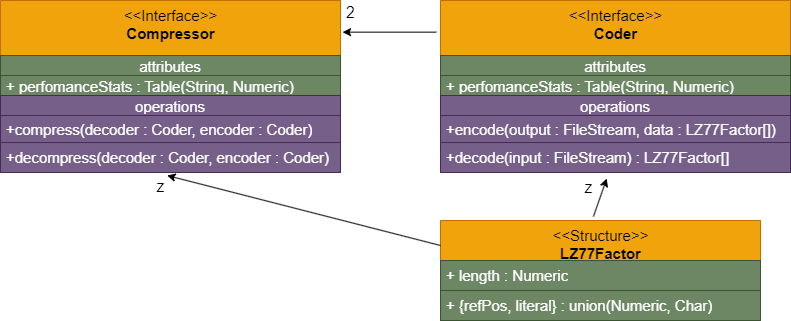
\includegraphics[scale=0.4]{Images/uml.png} \label{uml}
\end{figure}

Die in \ref{uml} dargestellte Klassenstruktur illustriert die grundlegende Abstraktion, die für die Implementierung der Algorithmen verwendet wurde. Compressor und
Coder beschreiben jeweils ein Interface bzw. ein Template, welches durch ein konkretes Kompressionsverfahren und einer Kodierung spezialisiert werden kann. Jegliche
Spezialisierungen teilen sich jedoch eine gemeinsame Definition eines Faktors im LZ77-Schema.

\subsection{Externe Bibliotheken}
Im Folgenden werden die genutzten externen Bibliotheken aufgelistet, die im Rahmen der Implementierung der Algorithmen, sowie deren Evaluation genutzt wurden.
\subsubsection{Malloc Count} \label{malloccount}
Malloc Count\cite{malloc_count} ist eine C++-Bibliothek, die es ermöglicht, Speicherallokationen und -freigaben auf dem Heap zu überwachen und zu messen. Im
Rahmen unserer Evaluation gibt uns diese Bibliothek die Spitze des allokierten Speichers innerhalb des Ausführung der Algorithmen aus.

\subsubsection{Unordered-Dense-Map} \label{unordereddense}
Die Unordered-Dense-Map\cite{unordered_dense} stellt eine hochperformante Hashtabelle dar, die insbesondere in der Dauer ihrer Suchoperationen gegenüber
der std::unordered\_map aus der Standardbibliothek deutlich trumpft. Dies Hashtabelle wurde in Approx.LZ77 und Approx.LZ77Par für die Speicherung der
RFPs in jeder Runde verwendet. Im Rahmen der Entwicklung von Approx.LZ77Par hat sich die Verwendung mehrerer Instanzen von Unordered-Dense-Map im Vergleich
zu anderen inherent parallelen Hashtabellen\cite{oneapi}\cite{sharded_map} als effizienter herausgestellt.

\subsubsection{LibSaiS}
Für die Implementierung der exakten LZ77-Faktorisierung, die als Referenzalgorithmus fungiert, wurde die Bibliothek LibSaiS\cite{libsais} zu Hilfe genommen. Diese
Bibliothek stellt eine effiziente Implementierung für die Konstruktion des Suffix-Arrays bereit.

\subsection{Parametrisierte Einstellung}
Falls nicht anders ausgewiesen wurden die Approximationsalgorithmen mit allen prakischen Optimierungen aus Kapitel 3.4 ausgeführt. Im Falle von Approx.LZ77Par
wurde die Ausführung standardmäßig mit 16 Threads durchgeführt. Unter Berücksichtung der verwendeten Eingabedaten wurde folgende Parameter für die 
Optimierungen festgelegt:
\begin{table} [ht]
    \centering
    \caption{Parameter und Einstellung für die Approximationsalgorithmen}
    \label{settings}
    \begin{tabular}{|c|c|}
        \hline
        \textbf{Einstellung} & \textbf{Wert} \\
        \hline
        DynEnd & Aktiv \\
        \hline
        DynStart & Aktiv \\
        \hline
        PreMatching & $r_{prematching}=r_{DynEnd}-3$ \\
        \hline
        ScanSkip & $k_{min}=3\%$ \\
        \hline
    \end{tabular}
\end{table}

\section{Messung}

\subsection{Eingabedaten}
Die folgenden Algorithmen wurden auf verschiedenen Dateien aus dem Pizza \& Chili-Corpus getestet. Die verwendeten Dateien decken verschiedene Kontexte und damit
Kompressionspotentiale ab.
\begin{table}[ht]
    \centering
    \caption{Auflistung der verwendeten Eingabedaten}
    \label{inputdata}
    \begin{tabular}{|c|c|c|c|c|}
        \hline
        \textbf{Datei} & \textbf{Größe} & \textbf{Alphabetgröße} & \textbf{Beschreibung} \\
        \hline
        \texttt{dna} & 200MB & 4 & DNA-Sequenzen \\
        \hline
        \texttt{english} & 200MB & 256 & Englische Texte \\
        \hline
        \texttt{proteins} & 200MB & 20 & Proteinsequenzen \\
        \hline
        \texttt{sources} & 200MB & 256 & Quellcode \\
        \hline
        \texttt{xml} & 200MB & 256 & XML-Dateien \\
        \hline
    \end{tabular}
\end{table}
In der Tabelle \ref{inputdata} sind die verwendeten Dateien aufgelistet. Die Größe der Dateien wurde auf 200MB beschränkt, um einen angemessenen Rahmen für die 
Laufzeitmessung zu erhalten.

\subsection{Messgrößen}

\subsubsection{Laufzeit}
Die Laufzeit der Algorithmen wurde innerhalb der Ausführung gemessen. Dabei wird die Zeitmessung nach dem Laden der Eingabedatei gestartet und mit dem vollständigen
Auffüllen der Faktorfolge beendet. Damit wird das Einlesen der Eingabe und eine eventuelle Kodierung der Ausgabe nicht in die Laufzeitmessung einbezogen. Diese Strategie
hat ihren Hintergrund in der Tatsache, dass die konkrete Ausprägung des Eingabe- und Ausgabestroms keine Aussagekraft über die Qualität der Kompression hat.

\subsubsection{Speicher}
Der Speicherverbrauch der Algorithmen wurde auch intern mithilfe einer externen Bibliothek \ref{malloccount} gemessen. Dabei wurden Speicherallokationen auf dem Heap 
überwacht und gemessen. Im Rahmen dieser Arbeit wurde die Spitze des allokierten Speichers im Zeitraum nach dem Einlesen der Eingabedatei und nach dem vollständigen 
Auffüllen der Faktorfolge gemessen. Zu Vergleichszwecken wird der Speicherverbrauch in Relation zur Eingabegröße angegeben.

\subsubsection{Kompressionsrate CR*} \label{cr}
Die Kompressionsrate wird neben der Anzahl der Faktoren zum Großteil von der verwendeten Kodierung bestimmt. Wie bereits erwähnt, sind wir in der Wahl der Kodierung
nicht beschränkt, sodass die Aussagekraft bezüglich der Qualität der Kompression eingeschränkt ist. Es ist jedoch zu beachten, dass Faktoren, die durch Approx.LZ77
erzeugt werden stets eine Zweierpotenz als Länge annehmen. Die binäre Repräsentation dieser Längen kann daher in Abhängigkeit von der gewählten Kodierung kompakt 
konstruiert werden. Um dieses Phänomen zu illustrieren, geben wir im Folgenden eine naive Kodierung vor, auf dessen Grundlage wir die Kompressionrate $CR*$ definieren.
\begin{equation}
    |K_{LZ77}(f)| = 1 + \begin{cases}
        2\log_2(n) & \text{falls } |f| > 1 \\
        9 & \text{sonst}
    \end{cases}
\end{equation}
Im Falle von LZ77 bestimmt ein Bit, ob es sich um eine Referenz oder ein einzelnes Zeichen handelt. Im Falle einer Referenz wird die Länge und die Position der Referenz
mithilfe von $\log_2(n)$ Bits kodiert. Im Falle eines einzelnen Zeichens wird die ASCII-Kodierung des Zeichens verwendet, die 8 Bits benötigt.
\begin{equation}
    |K_{Approx.LZ77}|= 1 + \begin{cases}
        \log_2(n)+\log_2(\log_2(n)) & \text{falls } |f| > 1 \\
        9 & \text{sonst}
    \end{cases}
\end{equation}
Im Falle von Approx.LZ77 kann die Länge mithilfe von $\log_2(\log_2(n))$ Bits kodiert werden, da die Länge anhand einer einzelnen Bitposition bestimmt wird.

\newpage
\subsection{Messwerte}

\begin{table}[ht]
    \centering
    \caption{Messwerte der Algorithmen auf verschiedenen Eingabedateien}
    \label{messwerte}
    \begin{tabular} { |c|c|c|c|c|c| }
        \hline
        \textbf{Eingabe} & \textbf{Algorithmus} & \textbf{Laufzeit[s]} & \textbf{Speicher[Byte]} & \textbf{FR} & \textbf{CR*} \\
        \hline
        & LZ77 & 15.40 & 20.00 & 9.98\% & 70.83\% \\
        proteins & Approx.LZ77 & 44.06 & 9.94 & 15.34\% & 63.95\% \\
        & Approx.LZ77Par & 6.99 & 10.21 & 15.34\% & 63.95\% \\
        \hline
        & LZ77 & 13.47 & 20.00 & 5.60\% & 38.75\% \\
        sources & Approx.LZ77 & 40.43 & 6.42 & 10.05\% & 40.14\% \\
        & Approx.LZ77Par & 6.49 & 5.90 & 10.05\% & 40.14\% \\
        \hline
        & LZ77 & 15.36 & 20.00 & 6.70\% & 47.24\% \\
        english & Approx.LZ77 & 51.00 & 7.06 & 10.42\% & 43.39\% \\
        & Approx.LZ77Par & 7.46 & 6.16 & 10.42\% & 43.39\% \\
        \hline
        & LZ77 & 14.89 & 20.00 & 6.66\% & 47.46\% \\
        dna & Approx.LZ77 & 30.10 & 8.38 & 10.71\% & 45.53\% \\
        & Approx.LZ77Par & 4.80 & 6.66 & 10.71\% & 45.53\% \\
        \hline
        & LZ77 & 13.02 & 20.00 & 3.42\% & 23.61\% \\
        xml & Approx.LZ77 & 29.38 & 3.46 & 6.62\% & 26.78\% \\
        & Approx.LZ77Par & 4.91 & 3.46 & 6.62\% & 26.78\% \\
        \hline
    \end{tabular}
\end{table}

\begin{figure}[ht]
    \centering
    \caption{Laufzeitmessung von LZ77, Approx.LZ77 und Approx.LZ77Par(16 Threads) auf verschiedenen Präfixen von proteins. Als Vergleichsmaß wurde 
    die lineare Regression der Kurven gestrichelt eingezeichnet.}
    \label{runtime}
    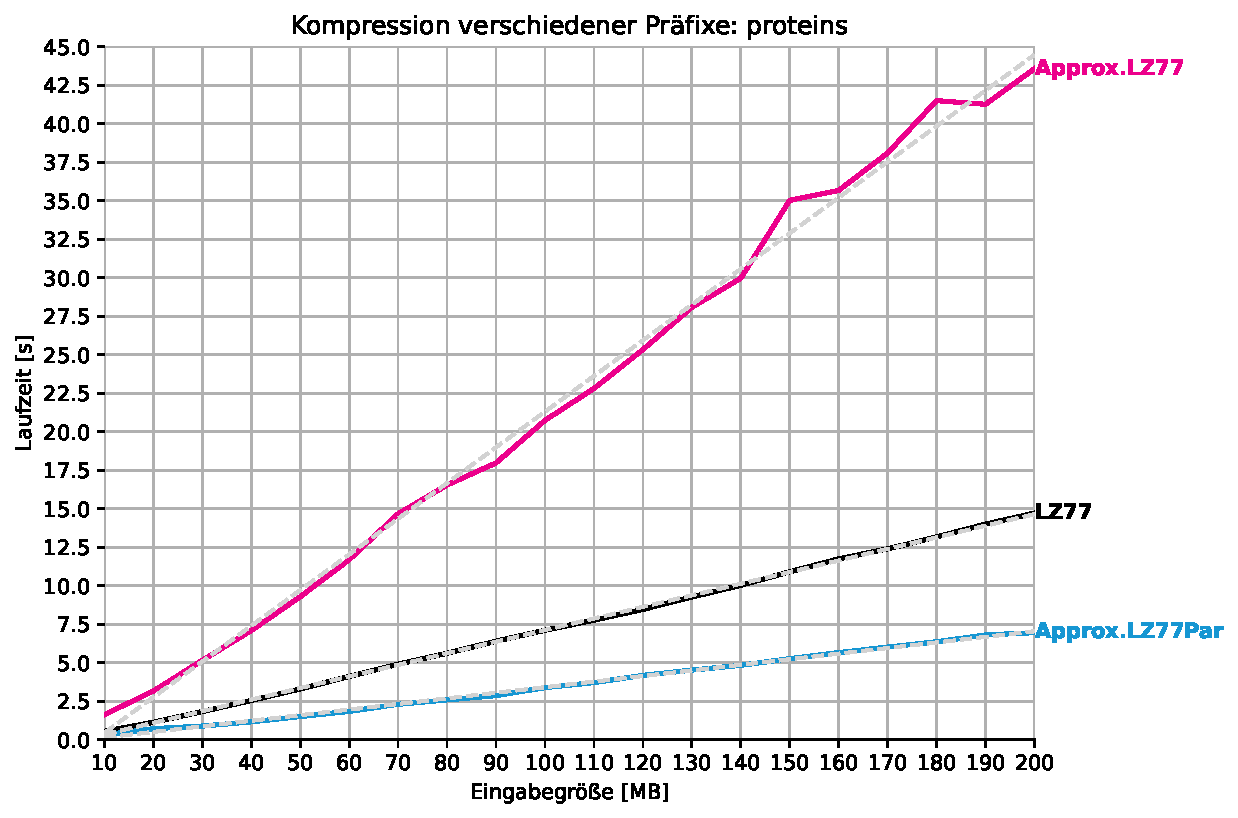
\includegraphics[scale=0.6]{Images/progressive_proteins.pdf}
\end{figure}
    
\begin{figure}[ht]
    \centering
    \caption{Laufzeitmessung von Approx.LZ77Par mit verschiedener Anzahl an Threads für proteins}
    \label{runtime_threads}
    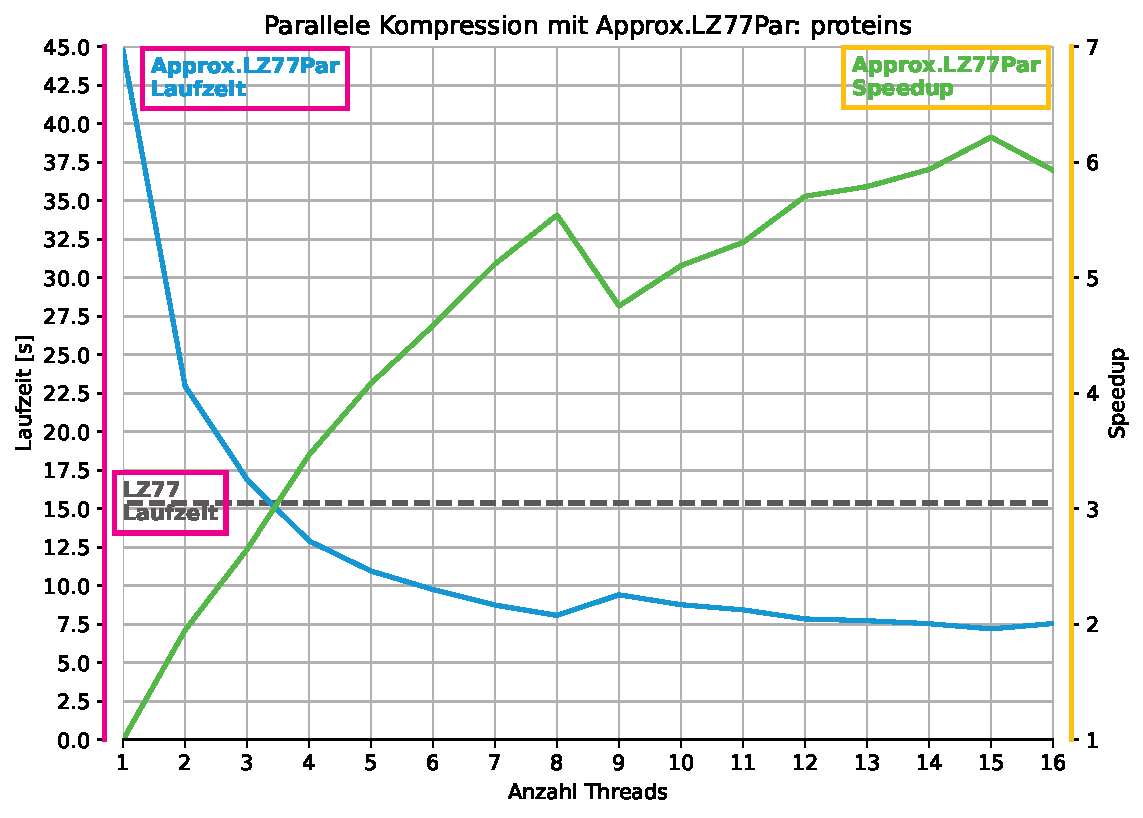
\includegraphics[scale=0.6]{Images/progressive_speedup_proteins.pdf}
\end{figure}

\begin{figure}[ht]
    \centering
    \caption{Speicherverbrauch von LZ77, Approx.LZ77 und Approx.LZ77Par(16 Threads) auf verschiedenen Präfixen von proteins. Aufgezeichnet wurde das Verhältnis
    von allokiertem Speicher zur Eingabegröße.}
    \label{memory}
    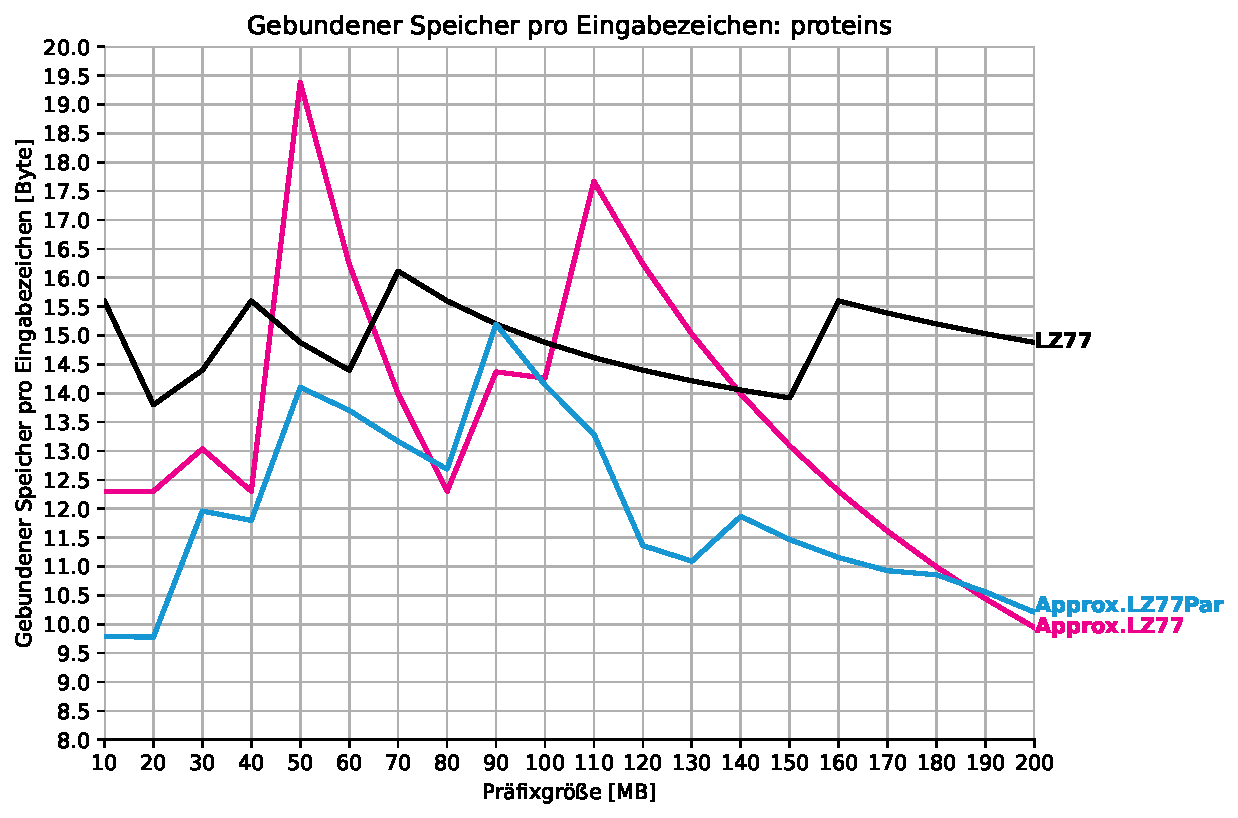
\includegraphics[scale=0.6]{Images/progressive_mem.pdf}
\end{figure}

\begin{figure}[ht]
    \centering
    \caption{Darstellung der Verteilung der Laufzeit der Subroutinen innerhalb jeder Runde im Falle einer Ausführung von Approx.LZ77 ohne jegliche Optimierungen \ref{sec:practopt}}
    \label{unopt}
    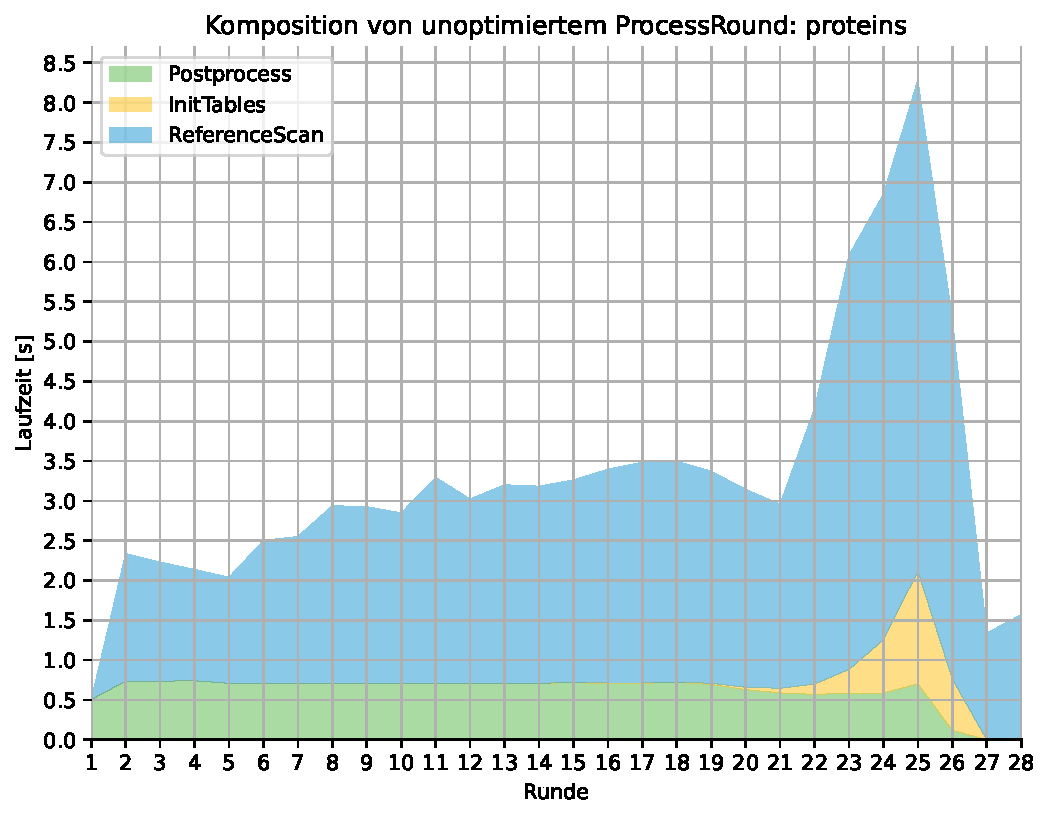
\includegraphics[scale=0.6]{Images/progressive_unopt_stack.pdf}
\end{figure}

\begin{figure}[ht]
    \centering
    \caption{Darstellung der Verteilung der Laufzeit der Subroutinen innerhalb jeder Runde im Falle einer Ausführung von Approx.LZ77 mit allen Optimierungen \ref{settings}}
    \label{opt}
    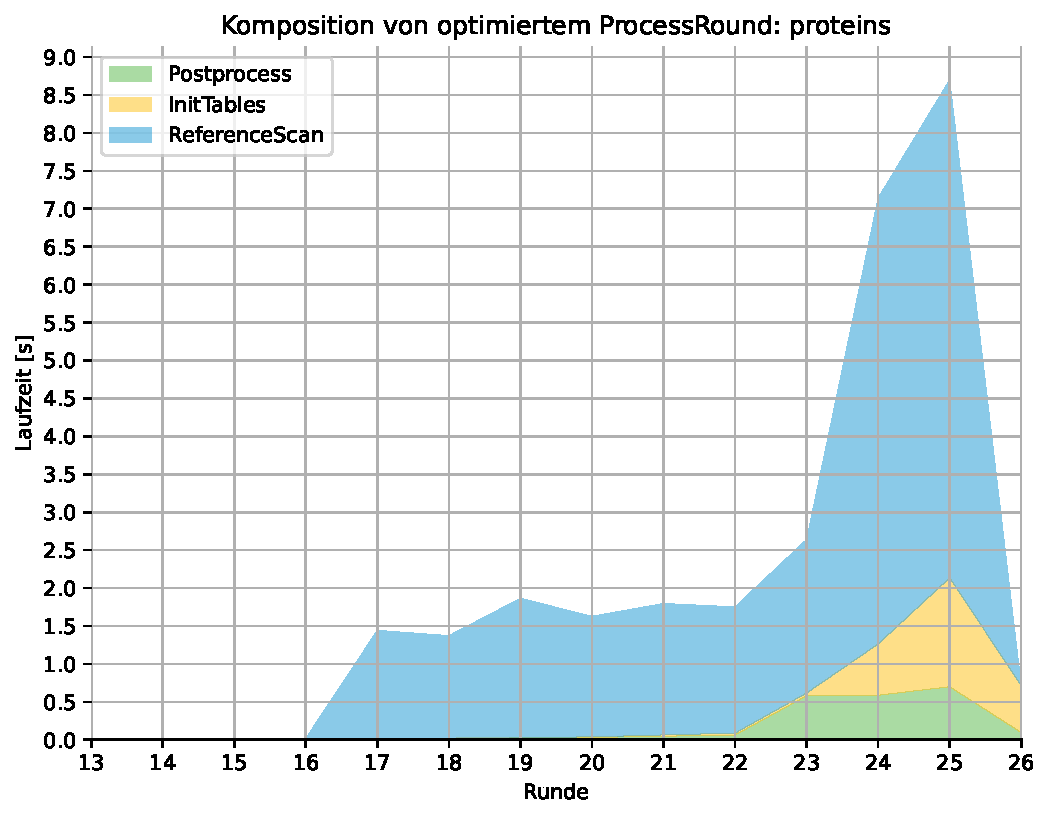
\includegraphics[scale=0.6]{Images/progressive_opt_stack.pdf}
\end{figure}

\section{Auswertung}
\subsection{LZ77}
Wie in Kapitel 3.1 beschrieben, zeigt der verwendete Algorithmus zur Generierung einer exakten LZ77-Faktorisierung ein lineares Verhalten bezüglich der Laufzeit.
Dies wird in Abbildung \ref{runtime} deutlich, wo die Laufzeitmessung von LZ77 auf verschiedenen Präfixen von proteins dargestellt ist. Die lineare Regression der
Kurven verdeutlicht das lineare Verhalten. Auch im Bezug auf die Speichernutzung wird das lineare Verhältnis zur Eingabegröße in Abbildung \ref{memory} deutlich.
Das Verhältnis von allokiertem Speicher zur Eingabegröße beträgt in nahezu allen Präfixen von proteins 20 Byte pro Eingabezeichen. Hiermit konnten wir die theoretische
Analyse des Laufzeit- und Speicherverhaltens empirisch bestätigen.

\subsection{Approx. LZ77}
In \ref{messwerte} wird deutlich, dass Approx. LZ77 dem exakten LZ77-Algorithmus in der Laufzeit und der Faktorrate stets deutlich unterlegen ist. Wie bereits in Kapitel
3.2 beschrieben, liegt der Fokus von Approx. LZ77 auf der Reduktion des Speicherverbrauchs. Weiterhin wurde eine schlechtere theoretische Laufzeitkomplexität von
$O(n\log n)$ gegenüber $O(n)$ von der exakten LZ77-Faktorisierung festgestellt. Die Messwerte in \ref{messwerte} bestätigen diese theoretische Analyse damit. Es ist 
jedoch zu beachten, dass Approx. LZ77 wie zu erwarten auch eine deutlich bessere Speichernutzung aufweist, wobei diese stark von der Eingabe abhängt. In Abbildung 
\ref{memory} wird deutlich, dass selbst verschiedene Präfixe einer Eingabedatei unterschiedliche relative Speichernutzungen aufweisen. Dies lässt sich auf ein 
unterschiedliches Maß der Redundanz in den Eingaben zurückführen. Die Kompressionsrate $CR*$ von Approx. LZ77 ist in \ref{messwerte} ebenfalls aufgeführt. Es ist 
zu erkennen, dass die Abweichung der Kompressionsrate von LZ77 in den meisten Fällen geringer ausfällt als die Abweichung der Faktorrate. Dies ist auf die in 
\ref{cr} beschriebene Eigenart der Kodierung zurückzuführen.

\subsection{Approx. LZ77 Optimierungen}
Die praktische Optimierungen aus Kapitel 3.4 wurden in der Evalutation von Approx.LZ77 und Approx.LZ77Par standardmäßig aktiviert. Um den Nutzen dieser Optimierungen
zu verdeutlichen wurden in \ref{unopt} und \ref{opt} die Auswirkungen auf die Laufzeiten der einzelnen Runden von Approx.LZ77 aufgezeichnet. Aufgrund der 
Optimierungen DynStart und DynEnd ist sofort ersichtlich, dass der Algorithmus einen großen Anteil der sonst nötigen Runden auslässt. Konkret werden die ersten 12 und
die letzten 2 Runden im Falle der Eingabe proteins ausgelassen. Dies bringt bereits eine signifikante Reduktion der Gesamtlaufzeit. Weiterhin fällt auf, dass die 
InitTables- und Postprocess-Routine im optimierten Fall deutlich weniger Zeit in Anspruch nehmen. Dies lässt sich auf die Anwendung von PreMatching zurückführen,
da in InitTables vorgefiltert werden und so weniger Einfügeoperationen stattfinden, sowie in Postprocess die Spaltung der Blöcke durch vorberechnete RFPs
beschleunigt wird. Dieser Effekt verfällt enstprechend nach der vorberechneten Runde, hier 24. Schließlich zeigt sich die Wirkung von ScanSkip in den Ausfällen
der ReferenceScan-Routine in den ersten vier und der letzten Runde. Die Kombination aus der Filterung durch PreMatching und der Eliminierung von Duplikaten in 
InitTables führt in beiden Fällen zu einer relativ kleinen RFPTable. In der Gesamtheit haben wir die Sinnhaftigkeit der Nutzung der Optimierungen in Approx.LZ77 
bestätigt. Die hier beschriebenen Effekte sind aufgrund des identischen Programmablaufs auch auf Approx.LZ77Par übertragbar.

\subsection{Approx. LZ77Par}
Im Bezug auf die Qualität der Kompression weist die Approx.LZ77Par keine Unterschiede zu Approx.LZ77 auf, was als Indiz für die Korrektheit der Implementierung
interpretiert werden kann. Die Laufzeitmessung in \ref{runtime} zeigt, dass Approx.LZ77Par mit 16 Threads eine deutlich bessere Laufzeit aufweist als Approx.LZ77.
Die Laufzeitmessung in \ref{runtime_threads} zeigt, dass die Laufzeit von Approx.LZ77Par von einer kleinen Anzahl an Threads stärker profitiert. Mit zunehmender 
Anzahl an Threads wird die Beschleunigung bzw. der Speedup geringer. Die resultierende Asymptote in der Laufzeitmessung ist auf externe Faktoren zurückzuführen,
wie der Bandbreite der Speicherzugriffe und Symptomen von False-Sharing. Der Speicherverbrauch von Approx.LZ77Par ist in \ref{memory} ebenfalls aufgezeichnet.
Es fällt auf, dass der Speicherverbrauch von Approx.LZ77Par im Vergleich zu Approx.LZ77 in den meisten Fällen leicht geringer ausfällt. 
Dies ist auf die Verwendung von mehreren Instanzen von Unordered-Dense-Map \ref{unordereddense} zurückzuführen, die aufgrund ihrer inhärenten Struktur einen 
geringen gesamten Speicherverbrauch aufweisen.
% Anhang
\appendix
% anhang.tex
\chapter{Weitere Informationen}
\section{Alternative Eingabedaten} \label{alternative}
Im Folgenden sind die vollständigen Laufzeitmessungen für die Eingabedaten, sources, english, dna und xml, aufgeführt. Während die absoluten Werte
der Laufzeit für die verschiedenen Eingabedaten variieren, zeigen die Kurven der Laufzeitmessungen eine ähnliche Tendenz.
\begin{figure} [H]
    \centering
    \caption{Laufzeitmessung von LZ77, Approx.LZ77 und Approx.LZ77Par(16 Threads) auf verschiedenen Präfixen von sources. Als Vergleichsmaß wurde 
    die lineare Regression der Kurven gestrichelt eingezeichnet.}
    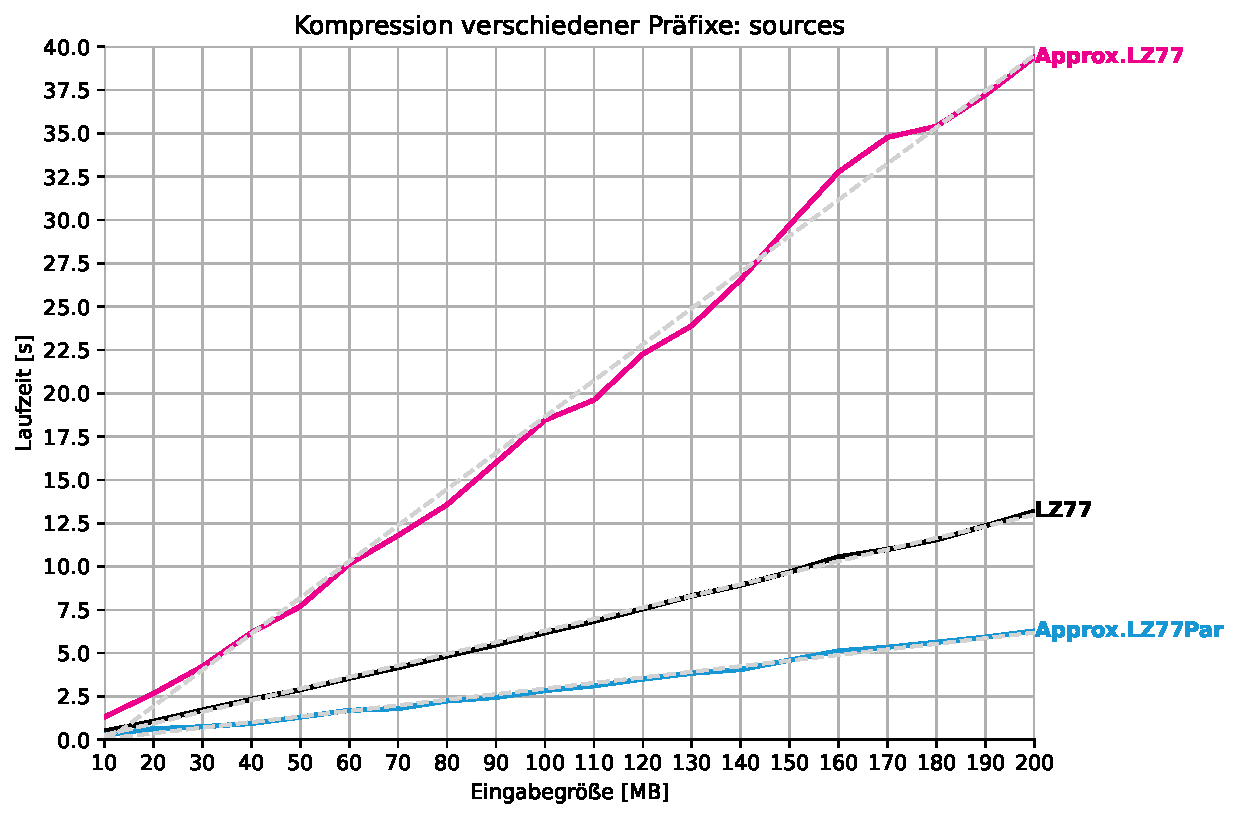
\includegraphics[scale=0.65]{Images/progressive_sources.pdf}
\end{figure}

\begin{figure}[H]
    \centering
    \caption{Laufzeitmessung von Approx.LZ77Par mit verschiedener Anzahl an Threads für sources}
    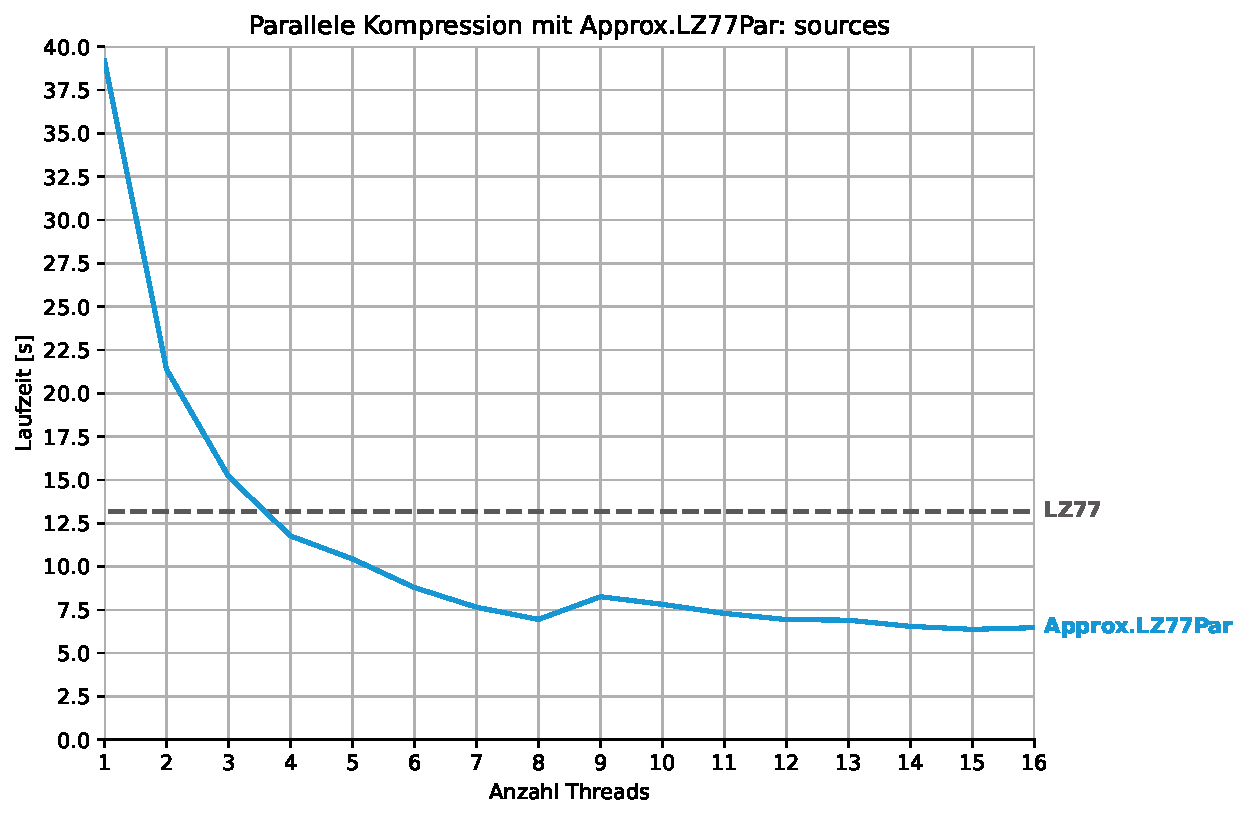
\includegraphics[scale=0.65]{Images/progressive_speedup_sources.pdf}
\end{figure}

\begin{figure}[H]
    \centering
    \caption{Laufzeitmessung von LZ77, Approx.LZ77 und Approx.LZ77Par(16 Threads) auf verschiedenen Präfixen von english. Als Vergleichsmaß wurde 
    die lineare Regression der Kurven gestrichelt eingezeichnet.}
    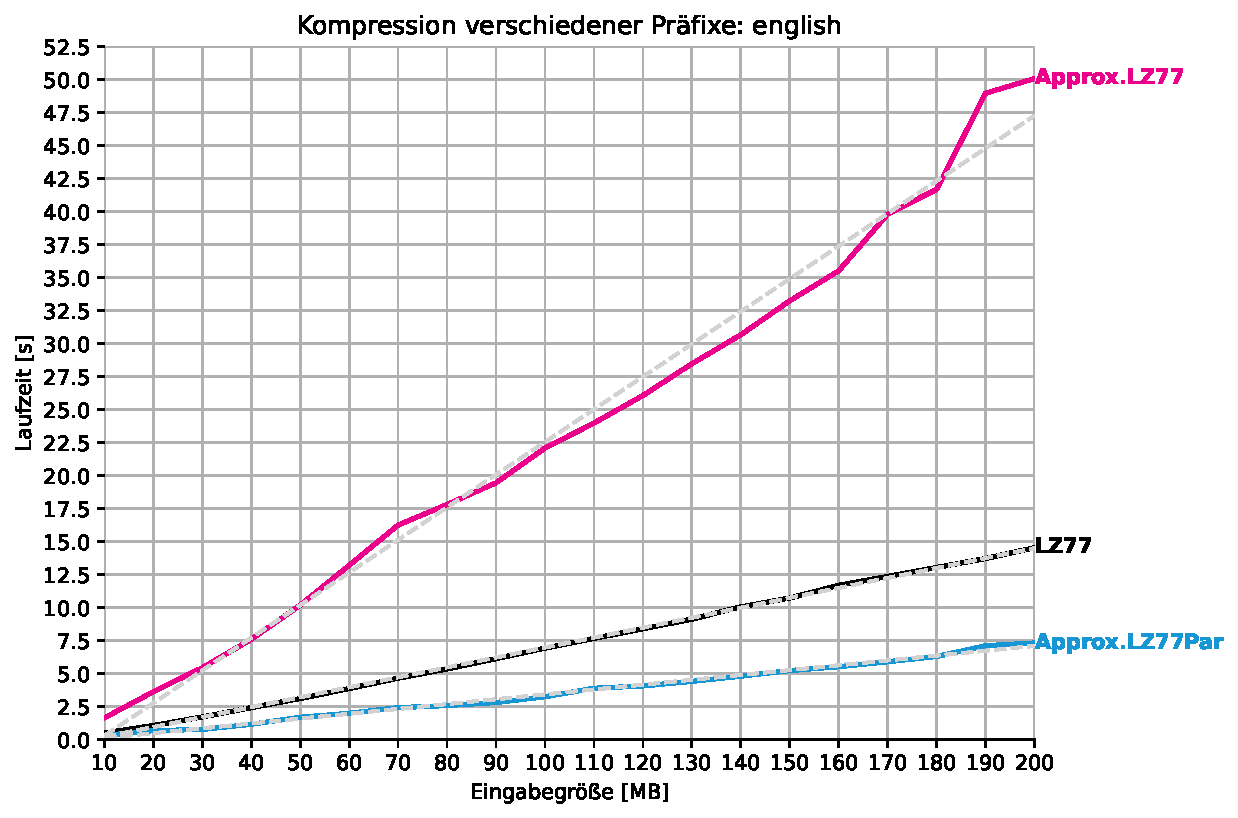
\includegraphics[scale=0.65]{Images/progressive_english.pdf}
\end{figure}

\begin{figure}[H]
    \centering
    \caption{Laufzeitmessung von Approx.LZ77Par mit verschiedener Anzahl an Threads für english}
    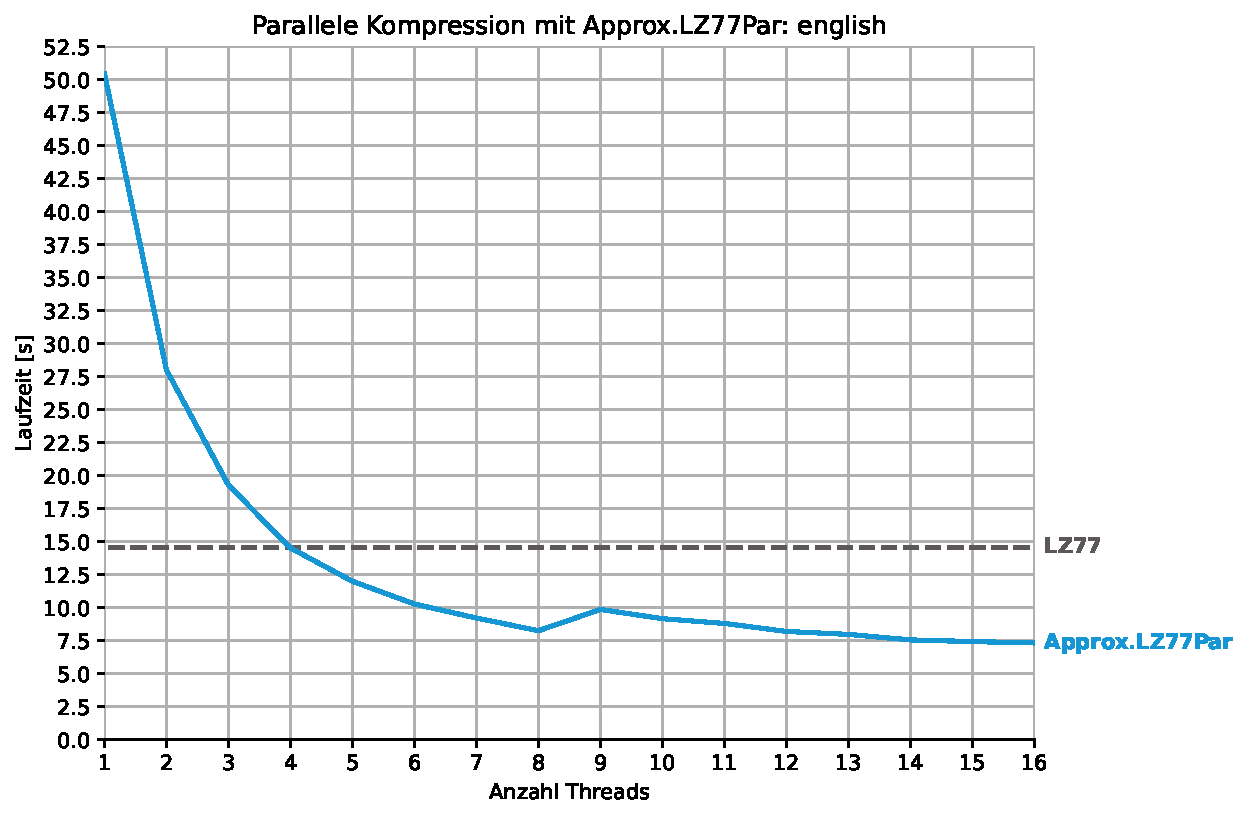
\includegraphics[scale=0.65]{Images/progressive_speedup_english.pdf}
\end{figure}

\begin{figure}[H]
    \centering
    \caption{Laufzeitmessung von LZ77, Approx.LZ77 und Approx.LZ77Par(16 Threads) auf verschiedenen Präfixen von dna. Als Vergleichsmaß wurde 
    die lineare Regression der Kurven gestrichelt eingezeichnet.}
    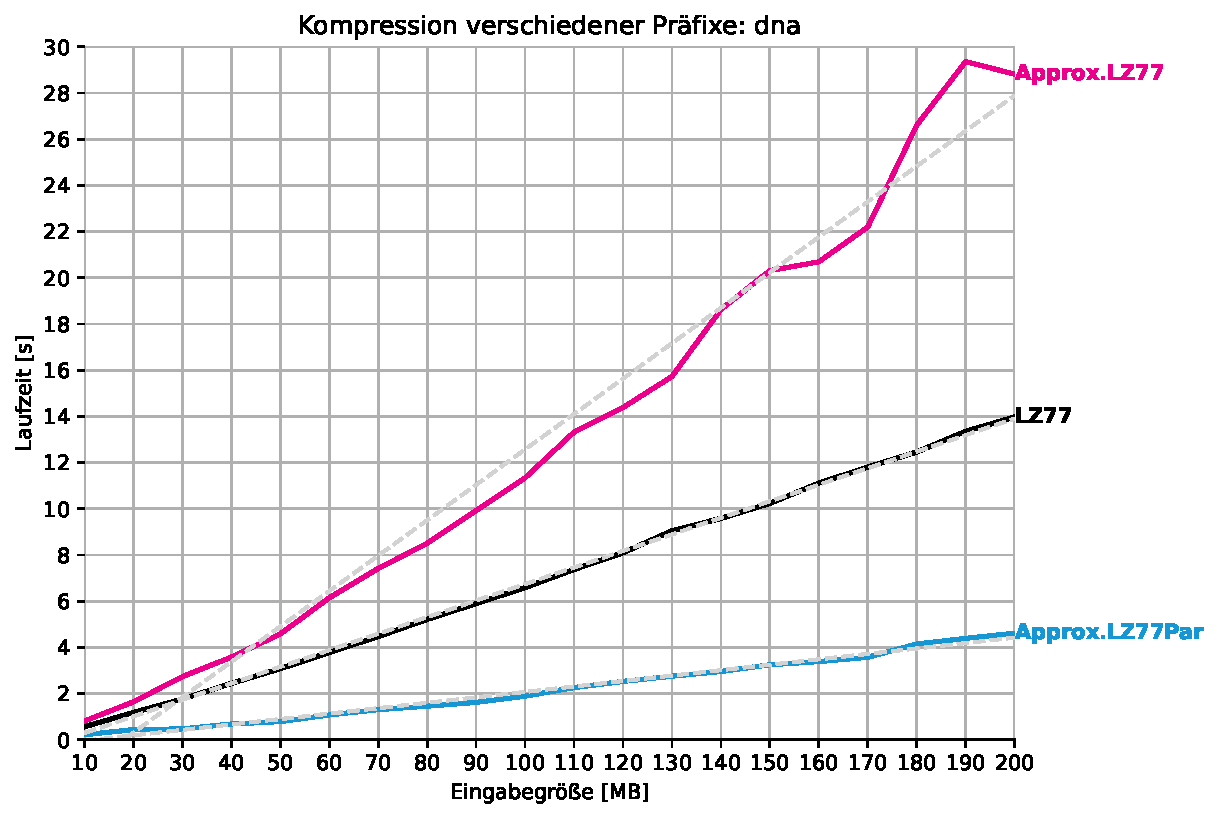
\includegraphics[scale=0.65]{Images/progressive_dna.pdf}
\end{figure}

\begin{figure}[H]
    \centering
    \caption{Laufzeitmessung von Approx.LZ77Par mit verschiedener Anzahl an Threads für dna}
    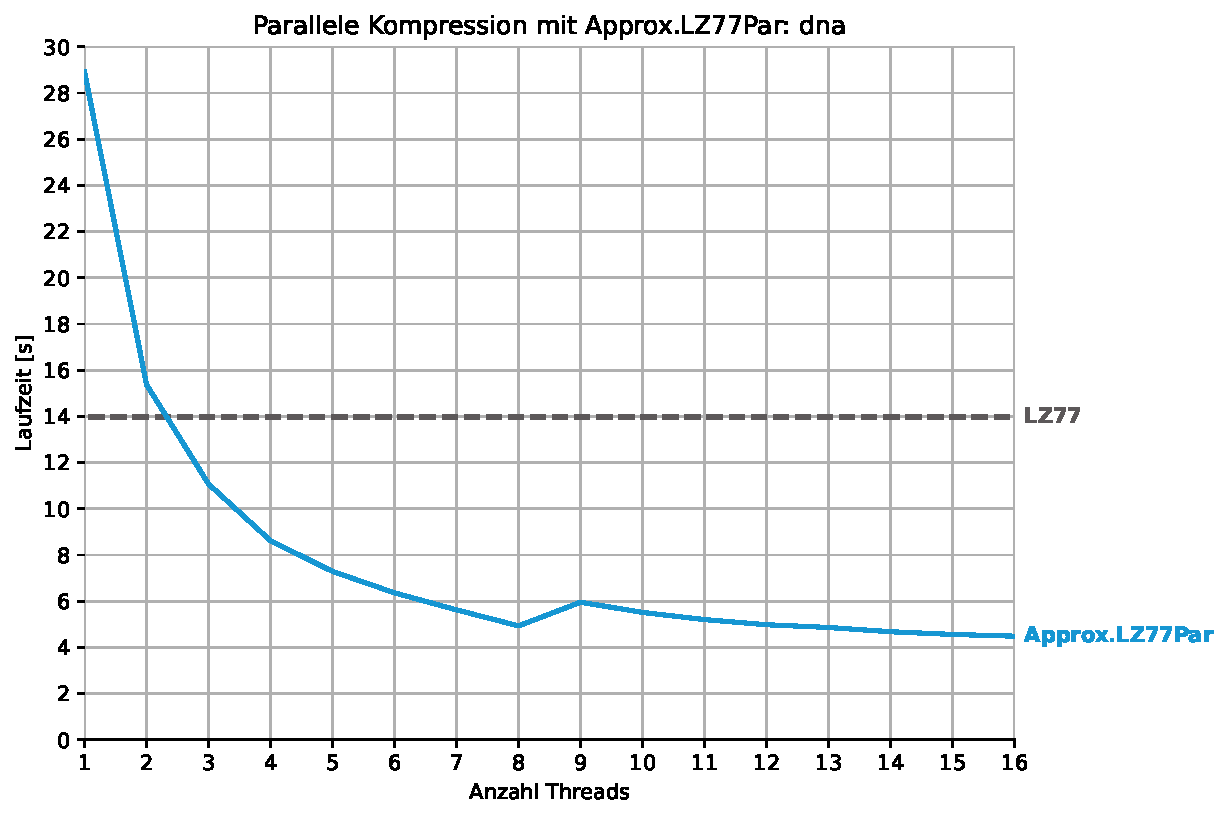
\includegraphics[scale=0.65]{Images/progressive_speedup_dna.pdf}
\end{figure}

\begin{figure}[H]
    \centering
    \caption{Laufzeitmessung von LZ77, Approx.LZ77 und Approx.LZ77Par(16 Threads) auf verschiedenen Präfixen von xml. Als Vergleichsmaß wurde 
    die lineare Regression der Kurven gestrichelt eingezeichnet.}
    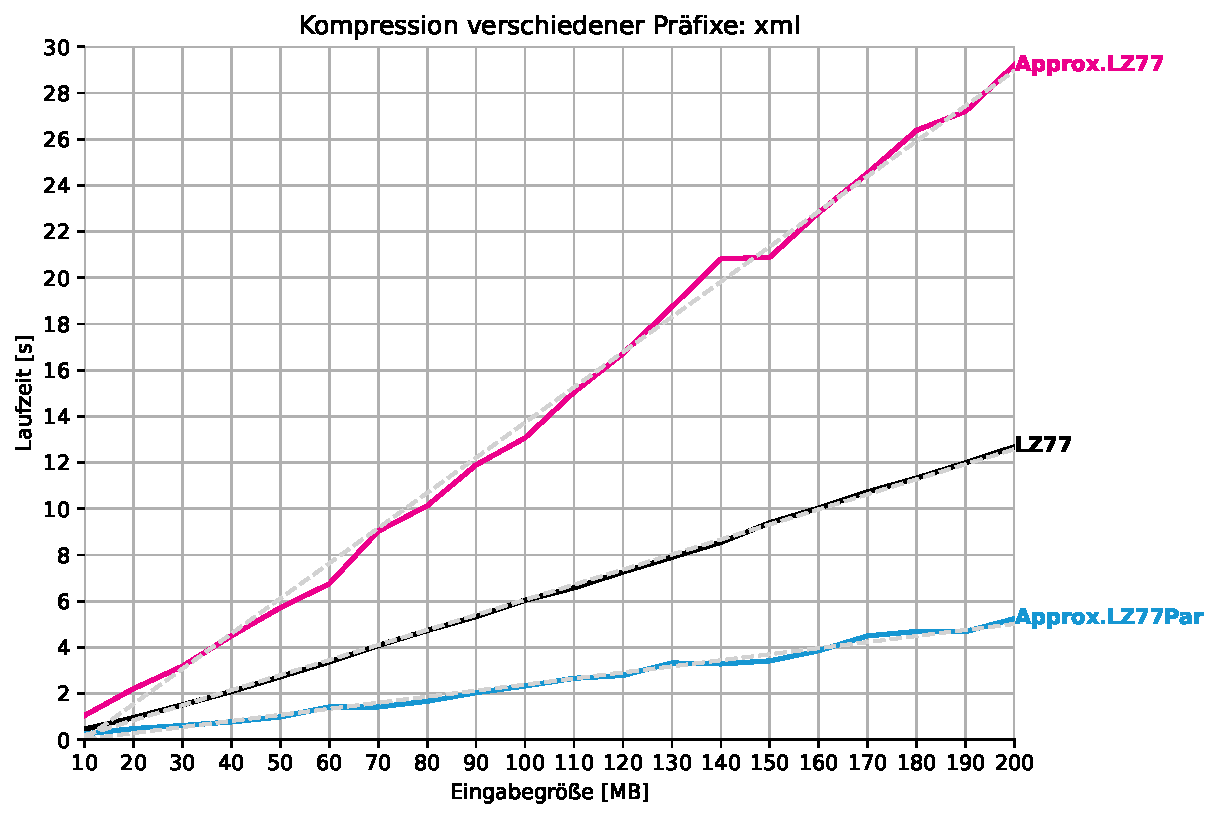
\includegraphics[scale=0.65]{Images/progressive_xml.pdf}
\end{figure}

\begin{figure}[H]
    \centering
    \caption{Laufzeitmessung von Approx.LZ77Par mit verschiedener Anzahl an Threads für xml}
    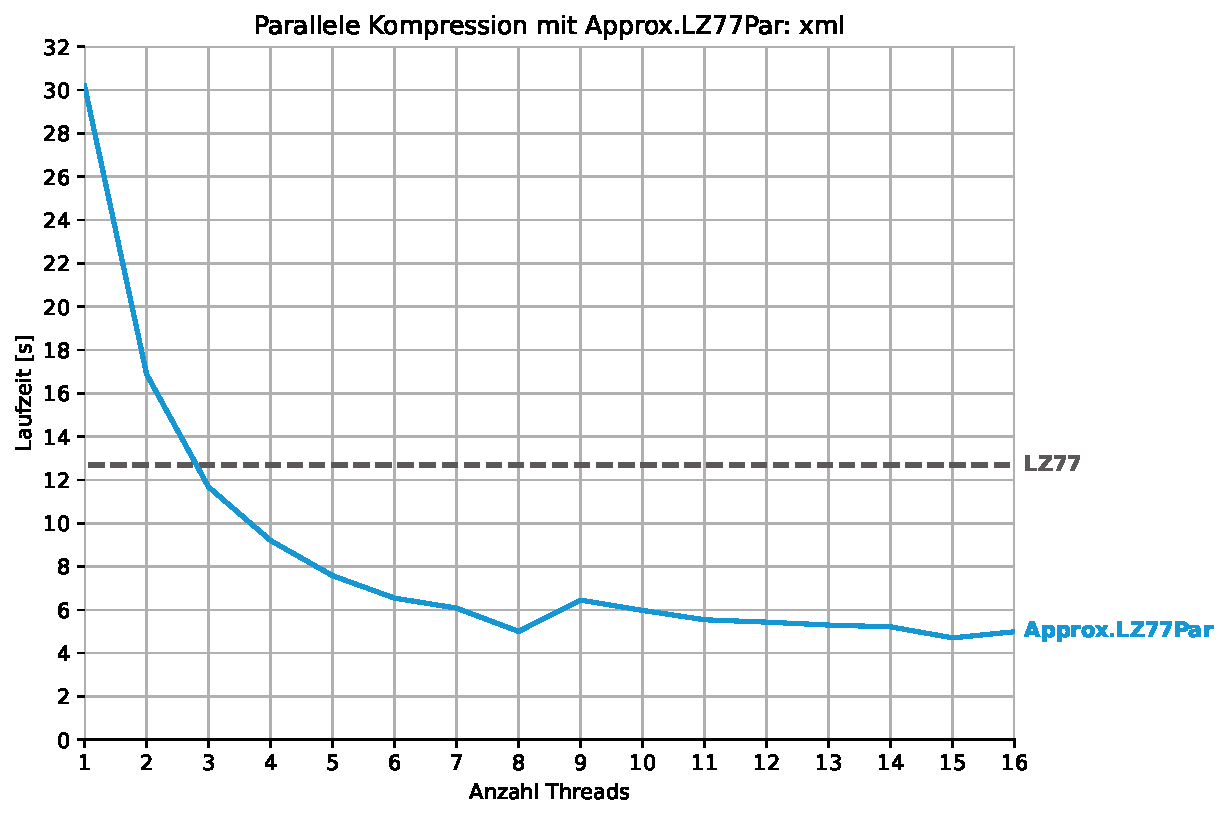
\includegraphics[scale=0.65]{Images/progressive_speedup_xml.pdf}
\end{figure}
\pagebreak
\section{Alternative Testumgebung}
Für die folgenden Messwerte wurden die Algorithmen auf einem Rechner mit einem AMD EYPC 7452 32-Core Prozessor mit 128 nutzbaren Threads ausgeführt.
Die Einstellungen der Algorithmen, die in \ref{settings} etabliert wurden, wurden beibehalten.

\begin{table}[ht]
    \centering
    \caption{Messwerte der Algorithmen auf verschiedenen Eingabedateien}
    \begin{tabular} { |c|c|c|c|c|c| }
        \hline
        \textbf{Eingabe} & \textbf{Algorithmus} & \textbf{Laufzeit[s]} & \textbf{Speicher} & \textbf{FR} & \textbf{CR*} \\
        \hline
        & LZ77 & 30.65 & 14.88 & 9.95\% & 70.92\% \\
        proteins & Approx.LZ77 & 64.46 & 9.94 & 15.34\% & 63.95\% \\
        & Approx.LZ77Par & 4.75 & 9.20 & 15.34\% & 63.95\% \\
        \hline
        & LZ77 & 28.38 & 13.44 & 5.50\% & 39.20\% \\
        sources & Approx.LZ77 & 62.35 & 6.42 & 10.05\% & 40.14\% \\
        & Approx.LZ77Par & 3.86 & 5.51 & 10.05\% & 40.14\% \\
        \hline
        & LZ77 & 33.59 & 13.44 & 6.66\% & 47.45\% \\
        english & Approx.LZ77 & 81.21 & 7.06 & 10.42\% & 43.39\% \\
        & Approx.LZ77Par & 4.30 & 5.95 & 10.42\% & 43.39\% \\
        \hline
        & LZ77 & 28.66 & 13.44 & 6.66\% & 47.46\% \\
        dna & Approx.LZ77 & 46.06 & 8.38 & 10.71\% & 45.53\% \\
        & Approx.LZ77Par & 3.52 & 6.13 & 10.71\% & 45.53\% \\
        \hline
        & LZ77 & 27.89 & 12.72 & 3.35\% & 23.89\% \\
        xml & Approx.LZ77 & 49.88 & 3.46 & 6.62\% & 26.78\% \\
        & Approx.LZ77Par & 2.91 & 3.28 & 6.62\% & 26.78\% \\
        \hline
    \end{tabular}
\end{table}
% Literaturverzeichnis
\bibliographystyle{gerplain}
\bibliography{References/diplom}
\addcontentsline{toc}{chapter}{\bibname}
% Erklaerung
\thispagestyle{myheadings}
\markboth{}{ERKLÄRUNG}
\addcontentsline{toc}{chapter}{Erklärung}
% erklaerung.tex
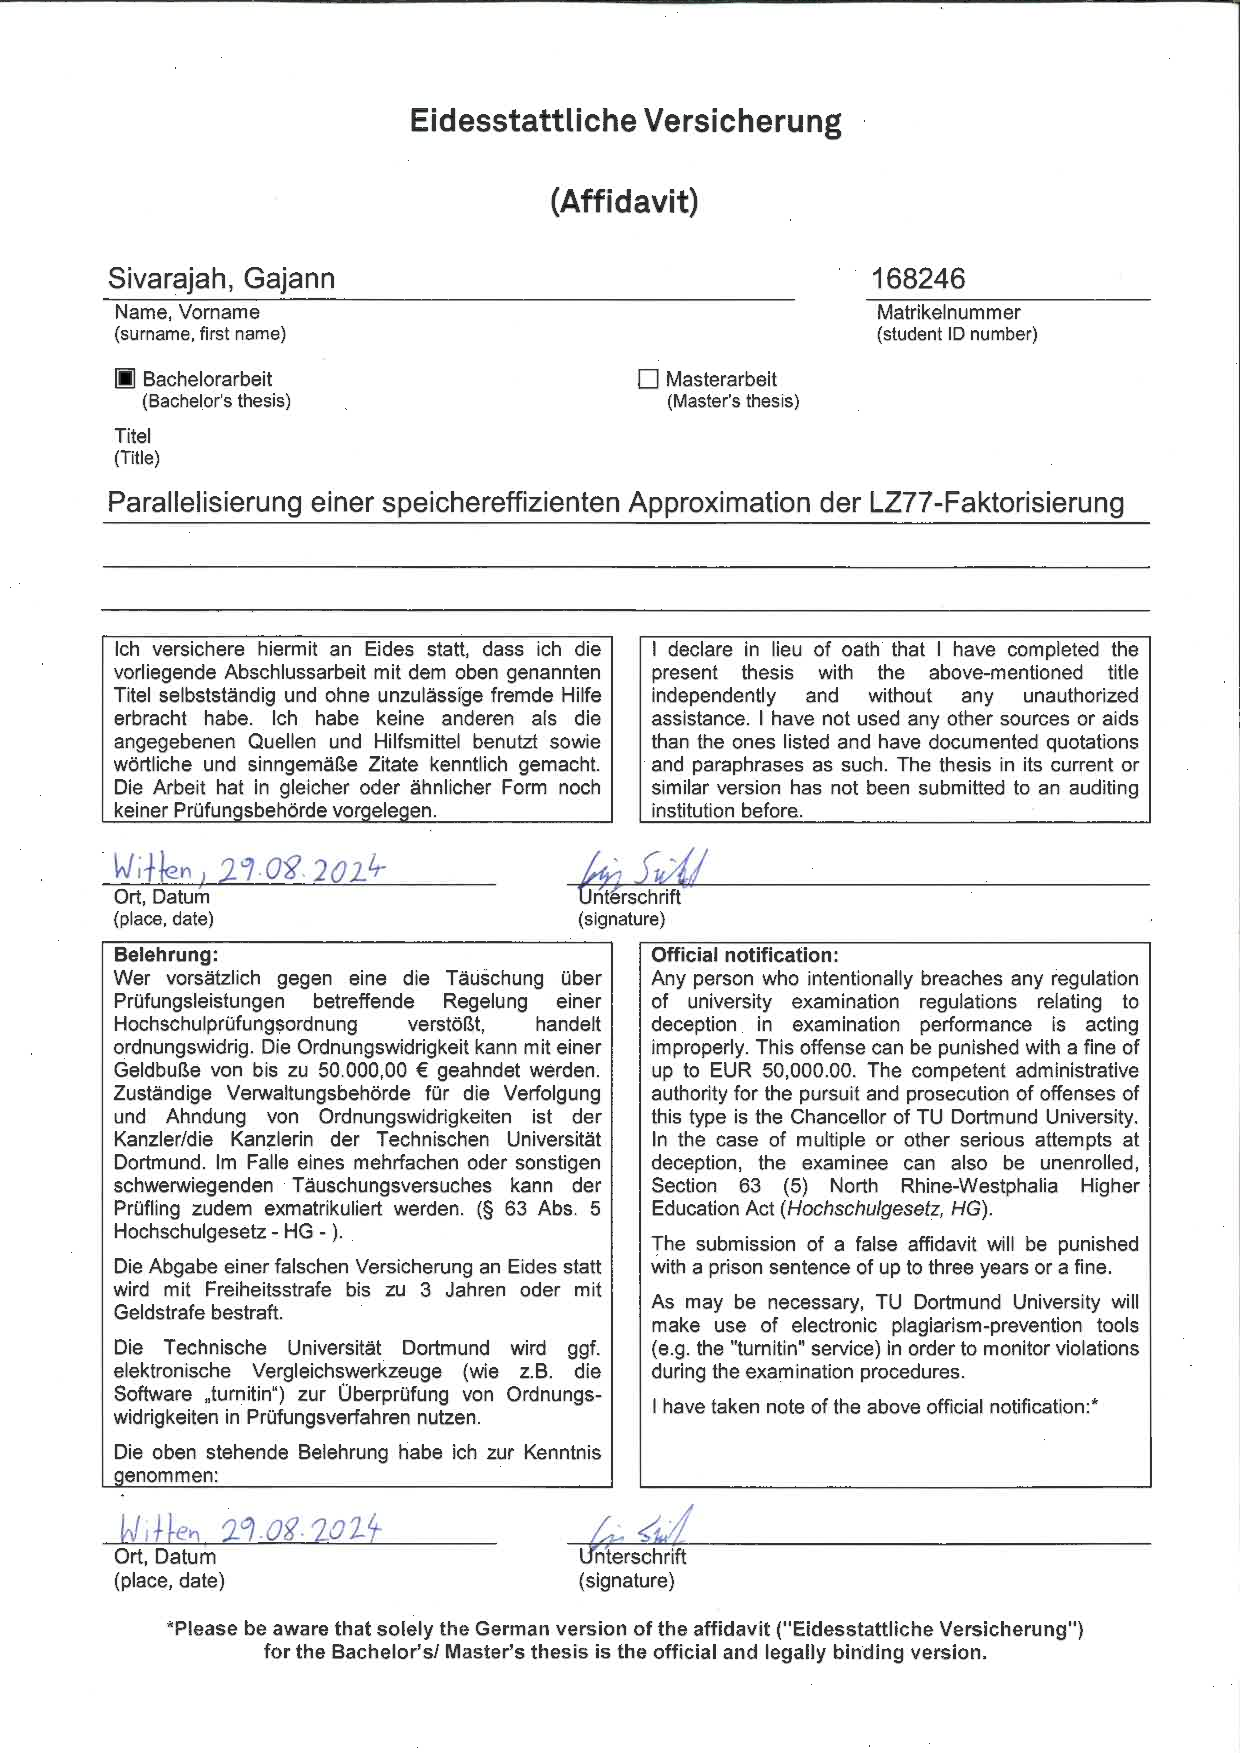
\includepdf{Chapters/Affidavit.pdf}
\cleardoublepage
\end{document}

